In this document we review the features of \texttt{oomph-lib}'s block 
preconditioning framework. We describe the functionality of the 
framework starting from the implementation of a simple block diagonal 
preconditioner. Then we introduce the LSC (Least Square Commutator) 
preconditioner for the Navier-Stokes equations~\cite{fastiterativesolvers}. 
Finally, we discuss the implementation of the augmented Lagrangian 
preconditioner for the solution of the constrained Navier-Stokes equations with
Lagrange multipliers.

The purpose of the block preconditioning framework (BPF) is to facilitate 
efficient implementation of the block preconditioners in a distributed 
environment. As such, it represents a software middleware which enables 
sytematic hierachical construction of block preconditioners for arbitrarily 
complex multiphysics problems by reusing the existing efficient preconditioners
for the constituent single physics sub-problems. At the same time the BPF hides
from the end user tedious implementation details associated with blocking of 
the Jacobian and the distribution of these blocks among the processors (these 
procedures involve the intricate communication with other parts of the library 
to obtain the necessary information). The operations performed by the BPF add 
only a minor computational overhead to the total solution time thus retaining 
asymptotically the same performance as the constituent scalar problem solvers 
(such as AMG). (CITE RICHARD THESIS AND PAGE NUMBER)

\section{ Theoretical Background\label{sec:theoretical_background}}
In \texttt{oomph-lib}, all problems are solved by Newton's method, which requires
the (if the problem is not linear, repeated) solution of linear systems of the 
form

\begin{equation}
J\;\mathbf{\delta x} = -\mathbf{r}
\label{eq:linear_system1}
\end{equation}
for the Newton correction $\mathbf{\delta x}$ where $J$ is the
Jacobian matrix and $\mathbf{r}$ is the vector of non-linear residuals. (Left) 
preconditioning represents a transformation of the original linear system 
\eqref{eq:linear_system1} to
\begin{equation*}
P^{-1}J\;\mathbf{ \delta x}=-P^{-1}\mathbf{r}
\end{equation*}
is introduced with the aim of accelerating the convergence of Krylov subspace 
iterative methods such as GMRES or CG (CITE saad). The application of the 
preconditioner requires the solution of a linear system
\begin{equation*}
P\mathbf{z}=\mathbf{y}
\end{equation*}
for $\mathbf{z}$ at each Krylov iteration.

Block preconditioning requires special enumeration schemes for the unknowns 
(equivalent to reordering the linear systems) where all the unknowns 
corresponding to each type of DOF are grouped together and enumerated 
consecutively. This leads to a natural block structure of the linear systems.
This process is equivalent to the following transformation
\begin{equation*}
  \underbrace{P_{\pi} A P_{\sigma}}_{\tilde{A}} \underbrace{P_{\sigma}^{\mathsf{T}}\mathbf{x}}_{\tilde{\mathbf{x}}}=\underbrace{P_{\pi}\mathbf{f}}_{\tilde{\mathbf{f}}}
\end{equation*}
where $P_{\pi}$ and $P_{\sigma}$ are the permutation matrices.

For instance, linear elasticity problems[CITE] involve the solid (the nodal 
positions in the solid domain) degrees of freedom (DOFs). Consider the 
two-dimensional case, we begin by reordering the linear system to group 
together the two types of DOF 
\begin{equation*}
\begin{bmatrix}
 J_{xx} & J_{xy} \\
 J_{yx} & J_{yy}
\end{bmatrix}
\begin{bmatrix}
 \mathbf{\delta x_x} \\
 \mathbf{\delta x_y} 
\end{bmatrix}
=
\begin{bmatrix}
 \mathbf{r_x} \\
 \mathbf{r_y}
\end{bmatrix},
\end{equation*}
then the block diagonal preconditioner of the form 
\begin{equation*}
P_{diag}=
\begin{bmatrix}
J_{xx}&     \\
      &J_{yy}
\end{bmatrix}
\end{equation*}
is obtained by omitting the off-diagonal blocks from the Jacobian [CITE].
The application of the preconditioner requires the exact or approximate 
solution of the linear system
\begin{equation*}
\begin{bmatrix}
J_{xx}& \\
      &J_{yy}
\end{bmatrix}
\begin{bmatrix}
\mathbf{z_x}\\
\mathbf{z_y}
\end{bmatrix}
=
\begin{bmatrix}
\mathbf{y_x}\\
\mathbf{y_y}
\end{bmatrix},
\end{equation*}
the two sub-blocks will be solved directly. The vector $\mathbf{y}$ is the 
linear residual at the current GMRES iteration.

%%%%%%%%%%%%%%%%%%%%%%%%%%%%%%%%%%%%%%%%%%%%%%%%%%%%%
%%% FRAMEWORK OVERVIEW
%%%%%%%%%%%%%%%%%%%%%%%%%%%%%%%%%%%%%%%%%%%%%%%%%%%%%
\section{ Framework Overview\label{sec:framework_overview}}
The above example shows that the application of block preconditioners
require several generic steps:
\begin{itemize}
\item The classification of the DOFs.
\item The application of subsidiary preconditioning operators.
\end{itemize}
The following subsections describe how these tasks are performed
within \texttt{oomph-lib}'s block preconditioning framework.

%%%% BLOCK PRECONDITIONABLE ELEMENTS
\subsection{Block Preconditionable Elements\label{sec:block_preconditionable_elements}}
The DOFs need to be classified into different types so that the BPF knows how
to group the DOFs which it then assemble into sub-matrices for the 
preconditioner blocks. The classification of DOFs is implemented at an 
elemental level. The class \texttt{GeneralisedElement} contains two broken 
virtual functions that must be re-implemented to label the DOFs with their 
type. The functions are:
\begin{itemize}
\item \texttt{GeneralisedElement::ndof\_types()} must return the number of DOF 
types associated with an element.
\item \texttt{GeneralisedElement::get\_dof\_numbers\_for\_unknowns(...)} 
must return a list of pairs comprising a map from global equation number to DOF
type for all unknowns in the element.
\end{itemize}
These are already implemented for many element types. For instance the 
two-dimensional FSI channel with leaflet problem has two types of element:
\begin{itemize}
\item \texttt{RefineableQTaylorHoodElement<2>} are the fluid elements. They have
three types of DOF; $x$-velocity DOFs are labelled \texttt{0}, $y$-velocity DOFs
are labelled \texttt{1} and the pressure DOFs are labelled \texttt{2}.
\item \texttt{FSIHermiteBeamElement} are the wall elements and have one type of
  DOF (the nodal position) labelled \texttt{0}.
\end{itemize}
The linear elasticity elements \texttt{MyLinearElasticityElement<DIM>} are made 
block-preconditionable with a wrapper around the element implemented in the 
driver code:
\lstset{numberfirstline=true,numberstyle=\scriptsize,breaklines=true, numbers=left, stepnumber=2, frame=single,basicstyle=\ttfamily\scriptsize, showstringspaces=false, language=C++}
\lstinputlisting[firstnumber=64,firstline=64, lastline=118]{./code/two_d_linear_elasticity_with_simple_block_diagonal_preconditioner.cc}
Thus, in the \texttt{MyLinearElasticityElement<2>} we have two types of DOF; 
corresponding to the $x$ and $y$ nodal displacements. They are classified as 
DOF types \texttt{0} and \texttt{1} respectively.

%%%% DOF TYPES AND BLOCK TYPES
\subsection{DOF types and block types\label{sec:dof_types_and_block_types}}
In the block diagonal preconditioner for the two-dimensional linear elasticity 
problem, there are two DOF types, there are also two block types. However, in 
more complicated preconditioners, such as the LSC preconditioner, there are 
more DOF types than there are block types. To see this, consider  using the 
LSC preconditioner on a 2D problem, we have two velocity DOF types, $x$ and 
$y$-velocities, and one pressure DOF type, $p$. But the LSC preconditioner 
works with velocity and pressure block types, the two velocity DOF types are 
combined to form one block type. Below we describe relationship between 
elemental DOF type classification, meshes, the block preconditioner DOF types, 
and block types:


\subsubsection{Elemental DOF type classification}

Each element classifies it's own DOF type in the function 
\texttt{get\_\allowbreak dof\_\allowbreak numbers\_\allowbreak for\_\allowbreak unknowns(...)}. In the case of 
\texttt{My\allowbreak Linear\allowbreak Elasticity\allowbreak Element<2>} elements, the DOF types are classified as 
\texttt{0} and \texttt{1}. For \texttt{Q\allowbreak TaylorHood\allowbreak Element<2>} 
elements, the DOF types are classified as \texttt{0} and \texttt{1} for the $x$
and $y$-velocities, and \texttt{2} for the pressure $p$, as depicted in Figure \ref{fig:2DTH_DOF_classification}.
\begin{figure}[H]
\centering
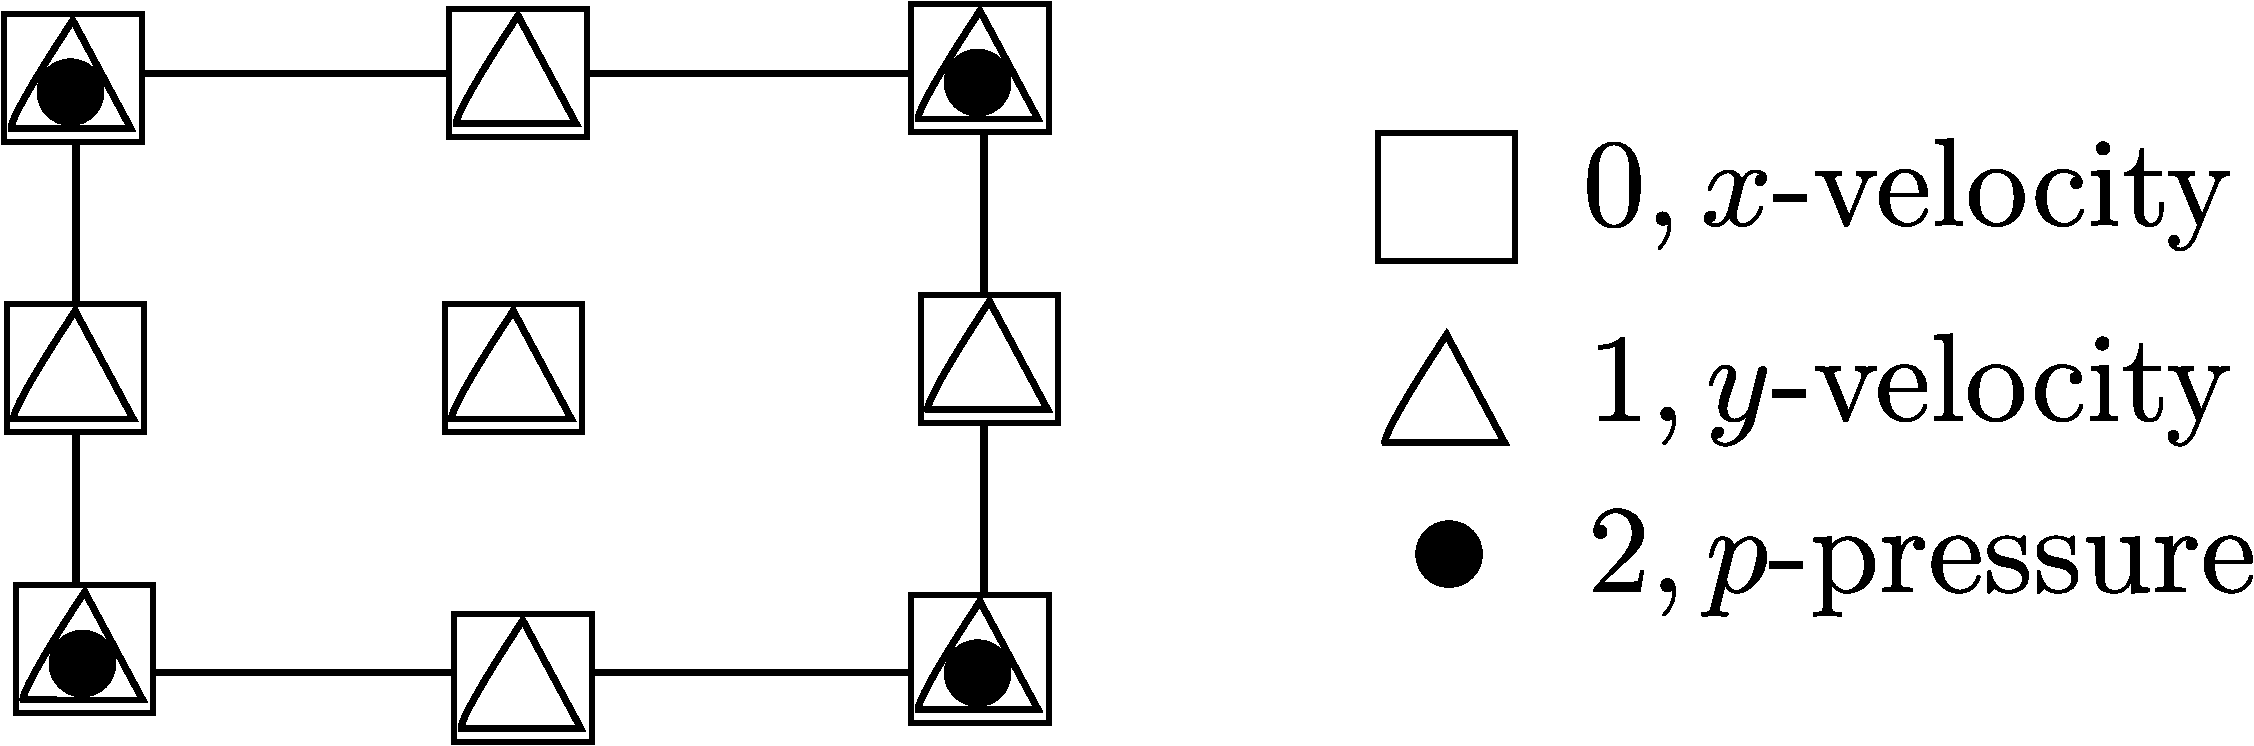
\includegraphics[width=0.8\textwidth]{./pic/taylorhood_dof_classification.pdf}
\caption{Elemental DOF type classification for \texttt{oomph-\allowbreak lib}'s
  \texttt{Q\allowbreak TaylorHood\allowbreak Element<2>} elements. The square,
  triangle and circle symbolises the DOF types within the element. Each element
  classifies it's DOFs locally.}
\label{fig:2DTH_DOF_classification}
\end{figure}

\subsubsection{The role of meshes}

Within the block preconditioning framework, each mesh acts as a container for 
a set of DOF type classifications. All elements in the same mesh \emph{must} 
return the same \texttt{ndof\_\allowbreak types()} value. If two different 
element types are in the same mesh, and their \texttt{ndof\_\allowbreak types()}
does indeed return the same number, then their elemental DOF type 
classifications will be treated as the same type. For example, recall in 
Figure \ref{fig:2DTH_DOF_classification} that the elemental DOF types 
classification for \texttt{Q\allowbreak TaylorHood\allowbreak Element<2>} 
elements are as follows:
\begin{itemize}
  \item \texttt{0} $x$-velocity
  \item \texttt{1} $y$-velocity
  \item \texttt{2} $p$-pressure
\end{itemize}
If we wish to constrain the flow along a boundary, we can attach the 
\texttt{Face\allowbreak Element}s 
\texttt{Impose\allowbreak Parallel\allowbreak Outflow\allowbreak Element<ELEMENT>} 
along the appropriate boundary as shown in the demo problem: Steady 
finite-Reynolds-number flow through an iliac bifurcation, these 
\texttt{Face\allowbreak Element}s classifies the `bulk' velocity DOF types 
as well as it's own DOF type as shown in Figure 
\ref{fig:2DFACE_DOF_classification}.
\begin{figure}[H]
\centering
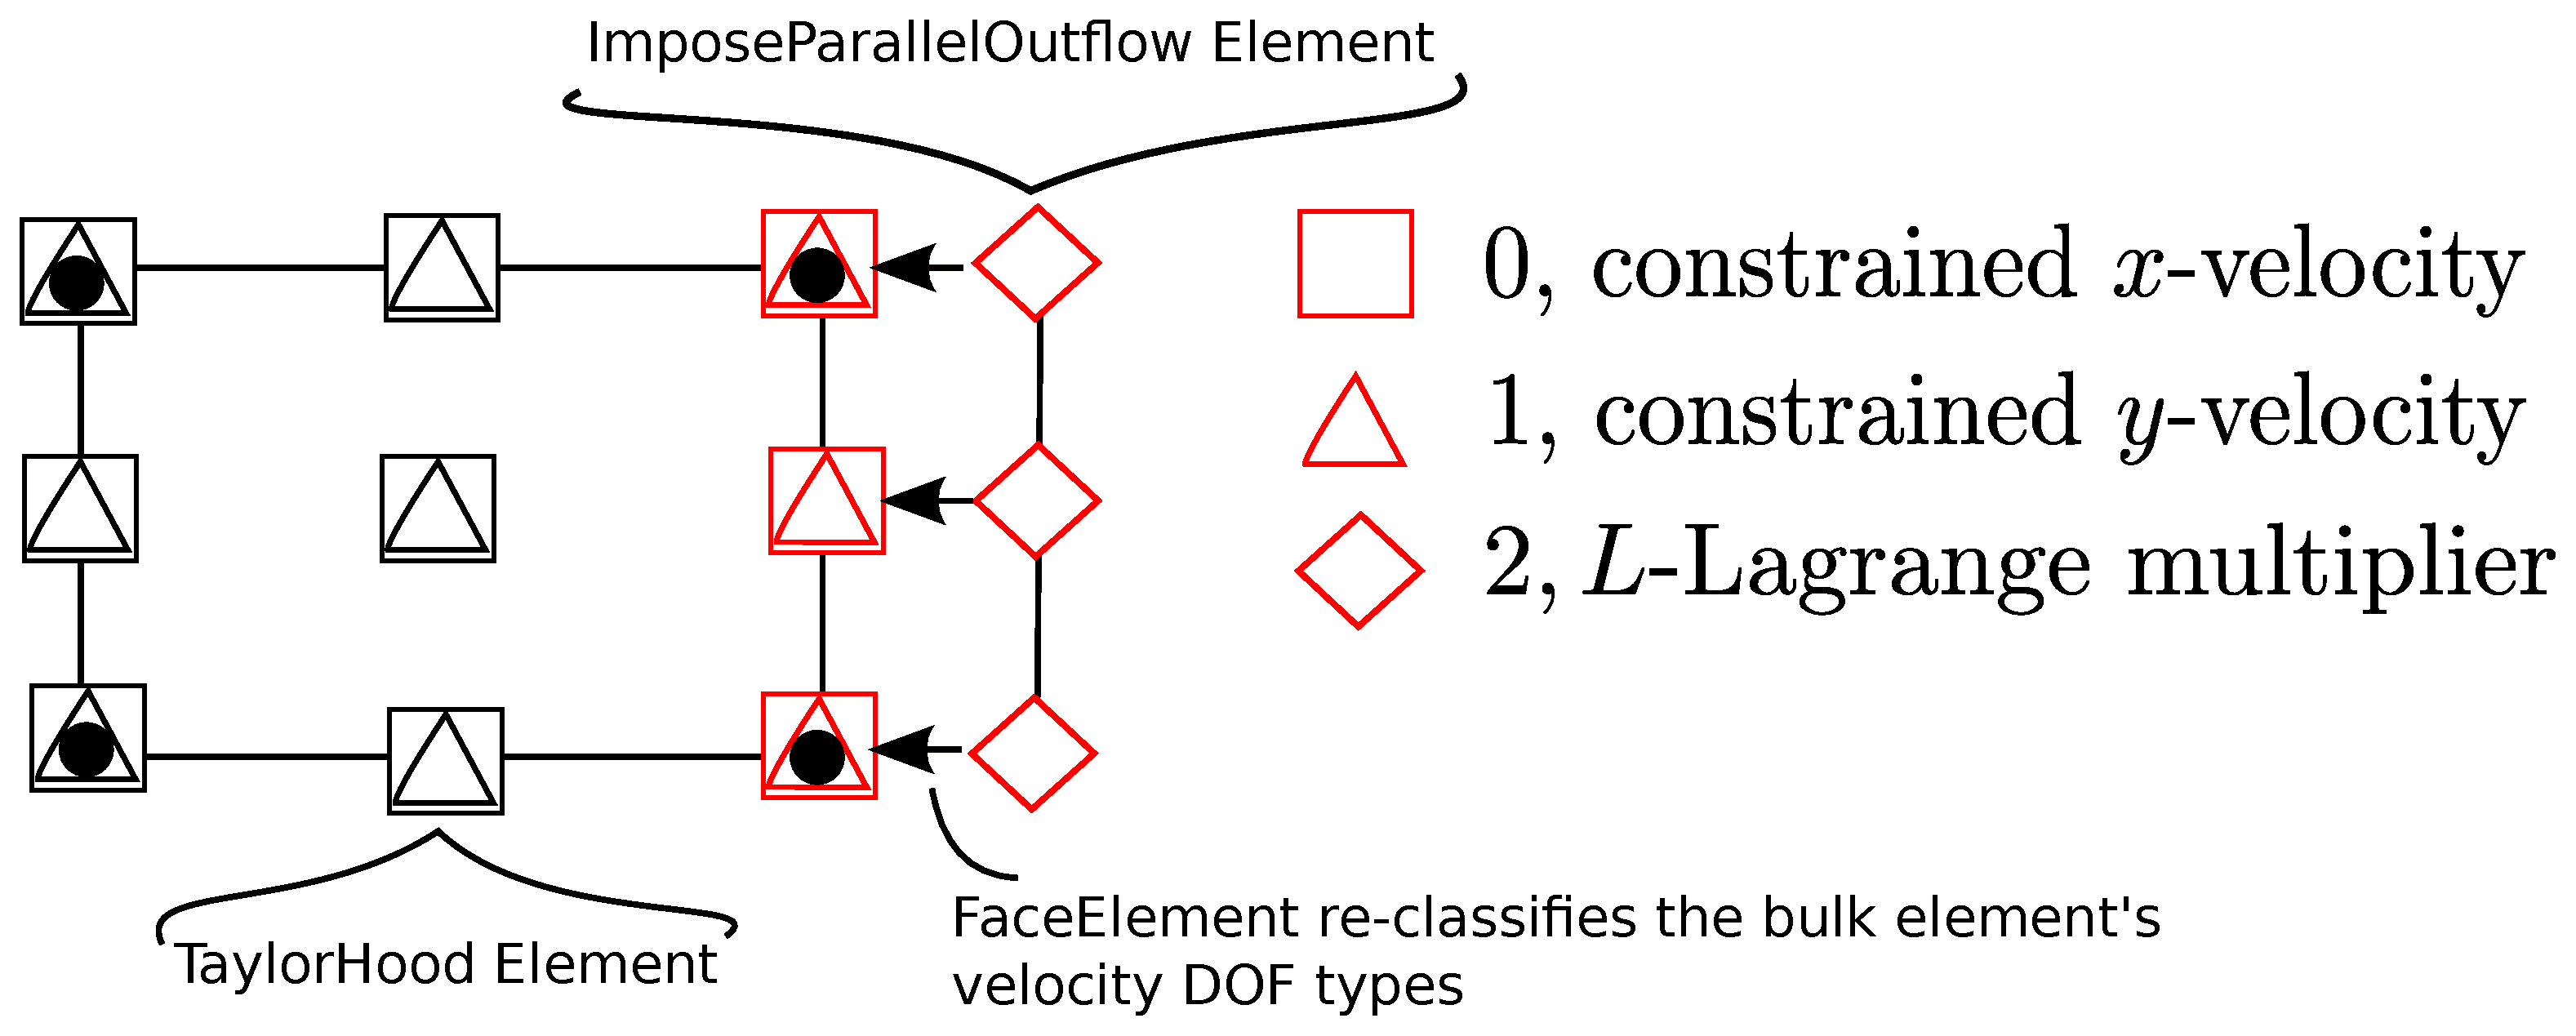
\includegraphics[width=0.9\textwidth]{./pic/faceelemenet_dof_classification.pdf}
\caption{Elemental DOF type classification for \texttt{oomph-\allowbreak lib}'s
  \texttt{Impose\allowbreak Parallel\allowbreak Outflow\allowbreak
    Element<ELEMENT>} elements. The black DOFs represents those classified by
  the TaylorHood element whilst the red DOFs are those which takes on the
  \texttt{Face\allowbreak Element} classification. Notice that this
  \texttt{Face\allowbreak Element} also (re-)classifies the velocity DOF types
  on the side of the bulk element it is attached to.}
\label{fig:2DFACE_DOF_classification}
\end{figure}

Although the \texttt{ndof\_\allowbreak types()} for these two different elements are the same,
there are clearly six distinct DOF types. To ensure that the block 
preconditioning framework treats these as different DOF types, we must have two
meshes for the two different type of elements. If we put the two elements types
in the same mesh, then the block preconditioning framework will not distinguish
between the two \texttt{0} elemental DOF types, i.e. $x$-velocity is the same as 
constrained $x$-velocity. The same applies to the remaining two elemental 
DOF types \texttt{1} and \texttt{2}. Within the block preconditioning framework, 
there is a built-in check to throw an error if a mesh passed to the framework 
contains multiple types of elements. This check can be avoided by setting the 
optional argument 
\texttt{allow\_\allowbreak multiple\_\allowbreak element\_\allowbreak type\_\allowbreak in\_\allowbreak mesh} 
when calling the function \texttt{set\_\allowbreak mesh(...)} to \texttt{true}. 
In this case, the framework will check if the \texttt{ndof\_\allowbreak types()} 
of all the elements of the same mesh are the same.

\subsubsection{Block preconditioner DOF types}
The information contained in different meshes allow the BPF to order the elemental
DOF types (note that the function \texttt{ndof\_\allowbreak types()} provides 
the block offset). For example, consider the above \texttt{vmtk} RAYFIX problem, 
the first mesh (the bulk mesh) contain elements with elemental DOF types 
\texttt{0}, \texttt{1} and \texttt{2} for the $x$, $y$-velocities and pressure
respectively. The second mesh (the surface mesh) contain elements with elemental
DOF types \texttt{0}, \texttt{1} and \texttt{2} for the $x$, $y$-constrained 
velocities and Lagrange multiplier respectively. Let $N$ be the 
number of meshes, $N_i$ be the number of elemental DOF types in mesh $i$,
$E_i = 0, \ldots N_i - 1$ be the elemental DOF types in mesh $i$, $B_{i,E_i}$ 
be the corresponding block preconditioner DOF types. Then the relationship 
between the block preconditioner DOF type $B_{i,E_i}$ and elemental DOF type
$E_i$ is given by
\begin{equation*}
  B_{i,E_i} = E_i + \sum_{i=0}^{N - 1} N_i, \quad \mbox{for } E_i = 0,\ldots N_i.
\end{equation*}
Figure \ref{fig:elemental_to_block_dof_classification} shows the mapping between
elemental DOF types and block preconditioner DOF types for the example above.
\begin{figure}[H]
\centering
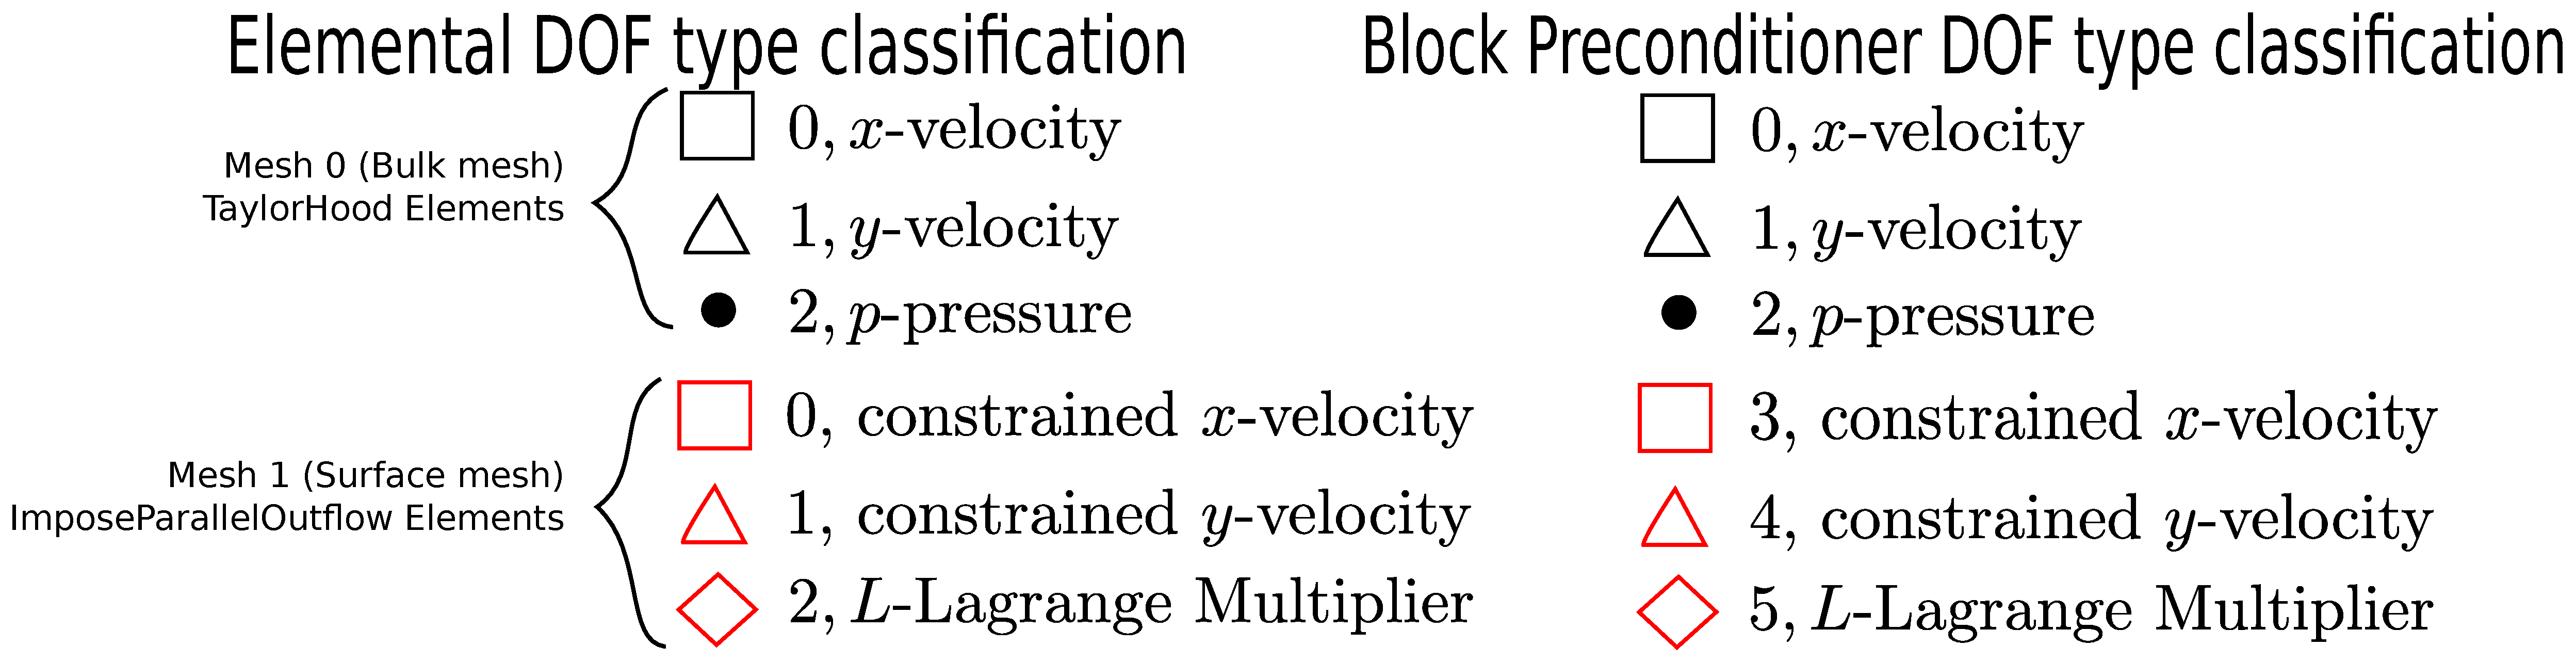
\includegraphics[width=1\textwidth]{./pic/elemental_to_block_dof_classification.pdf}
\caption{Relationship between the classification of elemental DOF types and
  preconditioner DOF types. Since the elemental DOF types are classified
  locally per element type, the meshes provide an offset used to differentiate
  the DOF types of different element types. DOFs can be classified more than
  once, the classification of the DOF will be the type given to it by the last
  element visited by the BPF which classified the DOF in question.}
\label{fig:elemental_to_block_dof_classification}
\end{figure}
It is important to note that within the BPF, when multiple meshes are used, the
block preconditioner DOF types admit to a two-level ordering: first by the mesh 
they belong to, and then by the elemental DOF type within the mesh. To this end, 
where the ordering of the block preconditioner DOF types matters (such as the 
LSC preconditioner), the block preconditioner should handle the ordering of the 
meshes, the user should use functions such as 
\texttt{set\_\allowbreak navier\_\allowbreak stokes\_\allowbreak mesh(...)}
in the case of the 
\texttt{Navier\allowbreak Stokes\allowbreak Schur\allowbreak Complement\allowbreak Preconditioner} 
since the LSC preconditioner know where the Navier-Stokes mesh need to be in 
the order of the meshes. We refer the ordering of the preconditioner DOF types, 
determined by the elemental DOF type and the ordering of the meshes, the 
\emph{natural ordering} of the preconditioner DOF types. For the above example, 
the natural ordering of the preconditioner DOF
types would be:
\begin{itemize}
 \item \texttt{0} $x$-velocity
 \item \texttt{1} $y$-velocity
 \item \texttt{2} $p$-pressure
 \item \texttt{3} constrained $x$-velocity
 \item \texttt{4} constrained $y$-velocity
 \item \texttt{5} $L$-Lagrange multiplier
\end{itemize}
Note: Each DOF can be classified more than once. If this is the case, then the 
classification will be the last mesh visited by the block preconditioning 
framework. This should not be an issue if you do not have discontinuous 
boundary conditions.

\subsubsection{Block types}
The block types are the blocks of sub-matrices the block preconditioner works 
with. Block types may contain more than one preconditioner DOF types or be as 
fine grain as the number of preconditioner DOF types. I.e. one or more 
preconditioner DOF types can make one block type (this is desirable if the 
physics of the underlying problem and the construction of the specific
preconditioner for it benefit from such classification). For example, in case 
of the LSC preconditioner (in 2D) we have three DOF types ($x$, $y$-velocities, 
and pressure), but the preconditioner only distinguishes between velocity and 
pressure DOF types, thus we have two block types (velocity block and pressure 
block). There can not be more block types than there are preconditioner DOF
types. 


Converting the elemental DOF types into preconditioner DOF types and then into 
block types is handled by the function \texttt{block\_\allowbreak setup(...)}.
We discuss the usage of this function in more detail later. The relationship 
between elemental DOF types, preconditioner DOF types and block types are 
summarised in Figure \ref{fig:dof_block_type_relations_crop}.
\begin{figure}[H]
\centering
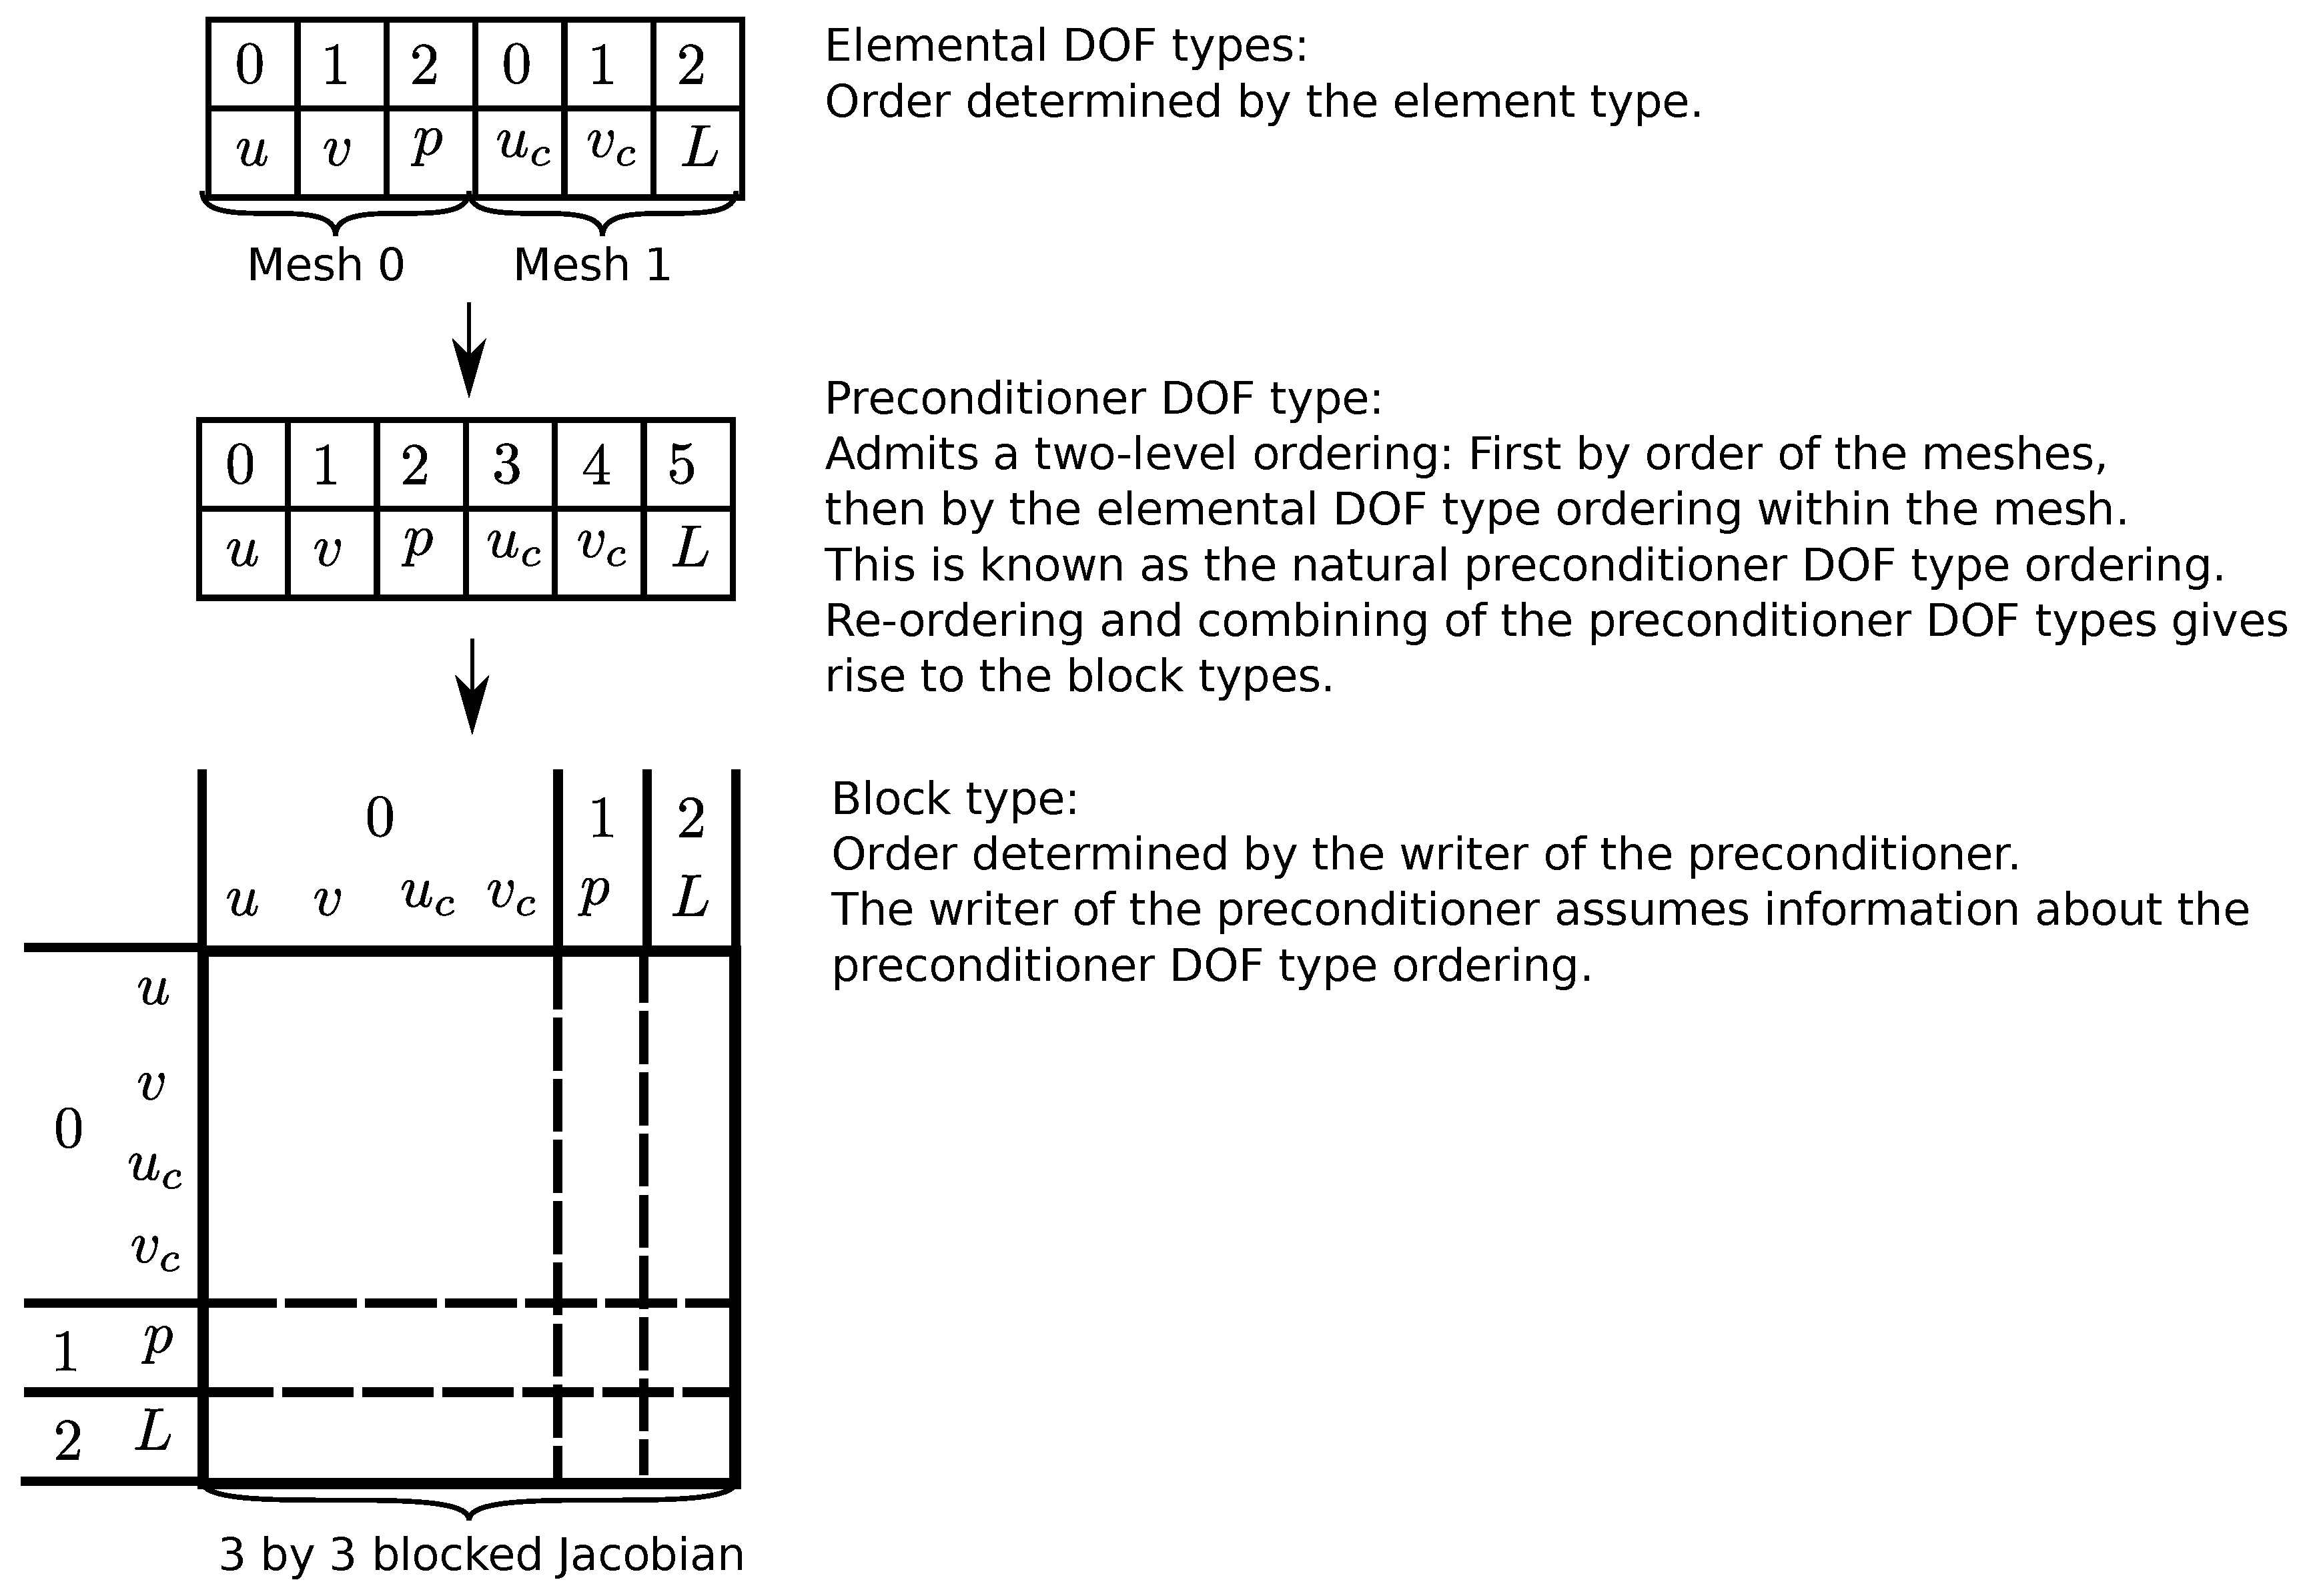
\includegraphics[width=1\textwidth]{./pic/dof_block_type_relations_crop.pdf}
\caption{Relationship elemental DOF types, preconditioner DOF types and block
  types. The arrow indicates the flow of dependency. The BPF requires the
  correct ordering of the meshes and elemental DOF types, which gives rise to
  the natural preconditioner DOF type ordering (this is the DOF type ordering
  assumed by the preconditioner). The BPF then re-orders and combine the
  relevant the DOF types to produce the required block types. With the block
  types set up, we are able to use the blocks for preconditioning. In the above
  example, block$(0,0)$ refers to the whole (combined) velocity block.}
\label{fig:dof_block_type_relations_crop}
\end{figure}


%%% MASTER AND SUBSIDIARY PRECONDITIONER
\subsection{Master and Subsidiary Preconditioners\label{sec:master_and_subsidiary_preconditioners}}
For each generic problem we perform the Jacobian blocking according to the
previously set rules and construct a preconditioner for that problem.  This
preconditioner is often referred to as the master preconditioner. Within this
preconditioner one needs to invert approximately some of the diagonal blocks or
the associated Schur compliments. This can be achieved by applying in a
systematic hierarchical manner with suitable preconditioners, referred to as
the subsidiary preconditioners. Each of subsidiary preconditioners, in turn,
can be implemented by introducing further subsidiary preconditioners. Such
decomposition of a master preconditioner leads to a tree-like structure (with a
master preconditioner in the root and the leaf nodes typically corresponding to
the scalar sub-problems solved by AMG). The BPF handles this recursive
tree-like definition of any generic preconditioner.

Consider again the LSC Navier-Stokes preconditioner. If we decide to approximate
the $\mathbf{F}$ block (the momentum block) by it's diagonal blocks, we can 
pass the block diagonal preconditioner (discussed in (Distributed) 
General-Purpose Block Preconditioners) to the LSC preconditioner to use as a 
subsidiary preconditioner via the function 
\texttt{set\_\allowbreak f\_\allowbreak preconditioner(...)}. We can do the 
same with the pressure system with the function 
\texttt{set\_\allowbreak p\_\allowbreak preconditioner(...)}. In this context, 
we refer to these preconditioners as subsidiary preconditioners. 
\texttt{Oomph-lib}'s block preconditioning framework facilitates the reuse of 
existing preconditioners as subsidiary preconditioners.

It is important to note that we do not need to consider the block structure of
subsidiary block preconditioners when developing master preconditioners.
However, the master preconditioner must be aware of the preconditioner DOF type
ordering assumed by subsidiary preconditioner. For example, if the LSC
preconditioner is a subsidiary preconditioner (as is the case of the Augmented
Lagrangian preconditioner preconditioner), the Augmented Lagrangian
preconditioner must ensure that the last preconditioner DOF type given to the
LSC preconditioner is the pressure DOF type, and the preconditioner DOF types
before that are the velocity DOF types.

For each problem, only one master preconditioner is defined and the remaining
preconditioners in the hierarchy are all considered to be subsidiary
preconditioners. Each subsidiary preconditioner holds a pointer to the
preconditioner one level higher in the hierarchy. Figure
\ref{fig:bpf_hierarchy_tree_crop} illustrates an example of a hierarchical tree
generated as a result of multiple levels of subsidiary preconditioning. Figure
\ref{fig:bpf_hierarchy_matrixstructure_crop} shows the structure of the
matrices and preconditioners for the same hierarchical tree as Figure
\ref{fig:bpf_hierarchy_tree_crop}.

\begin{figure}[H]
\centering
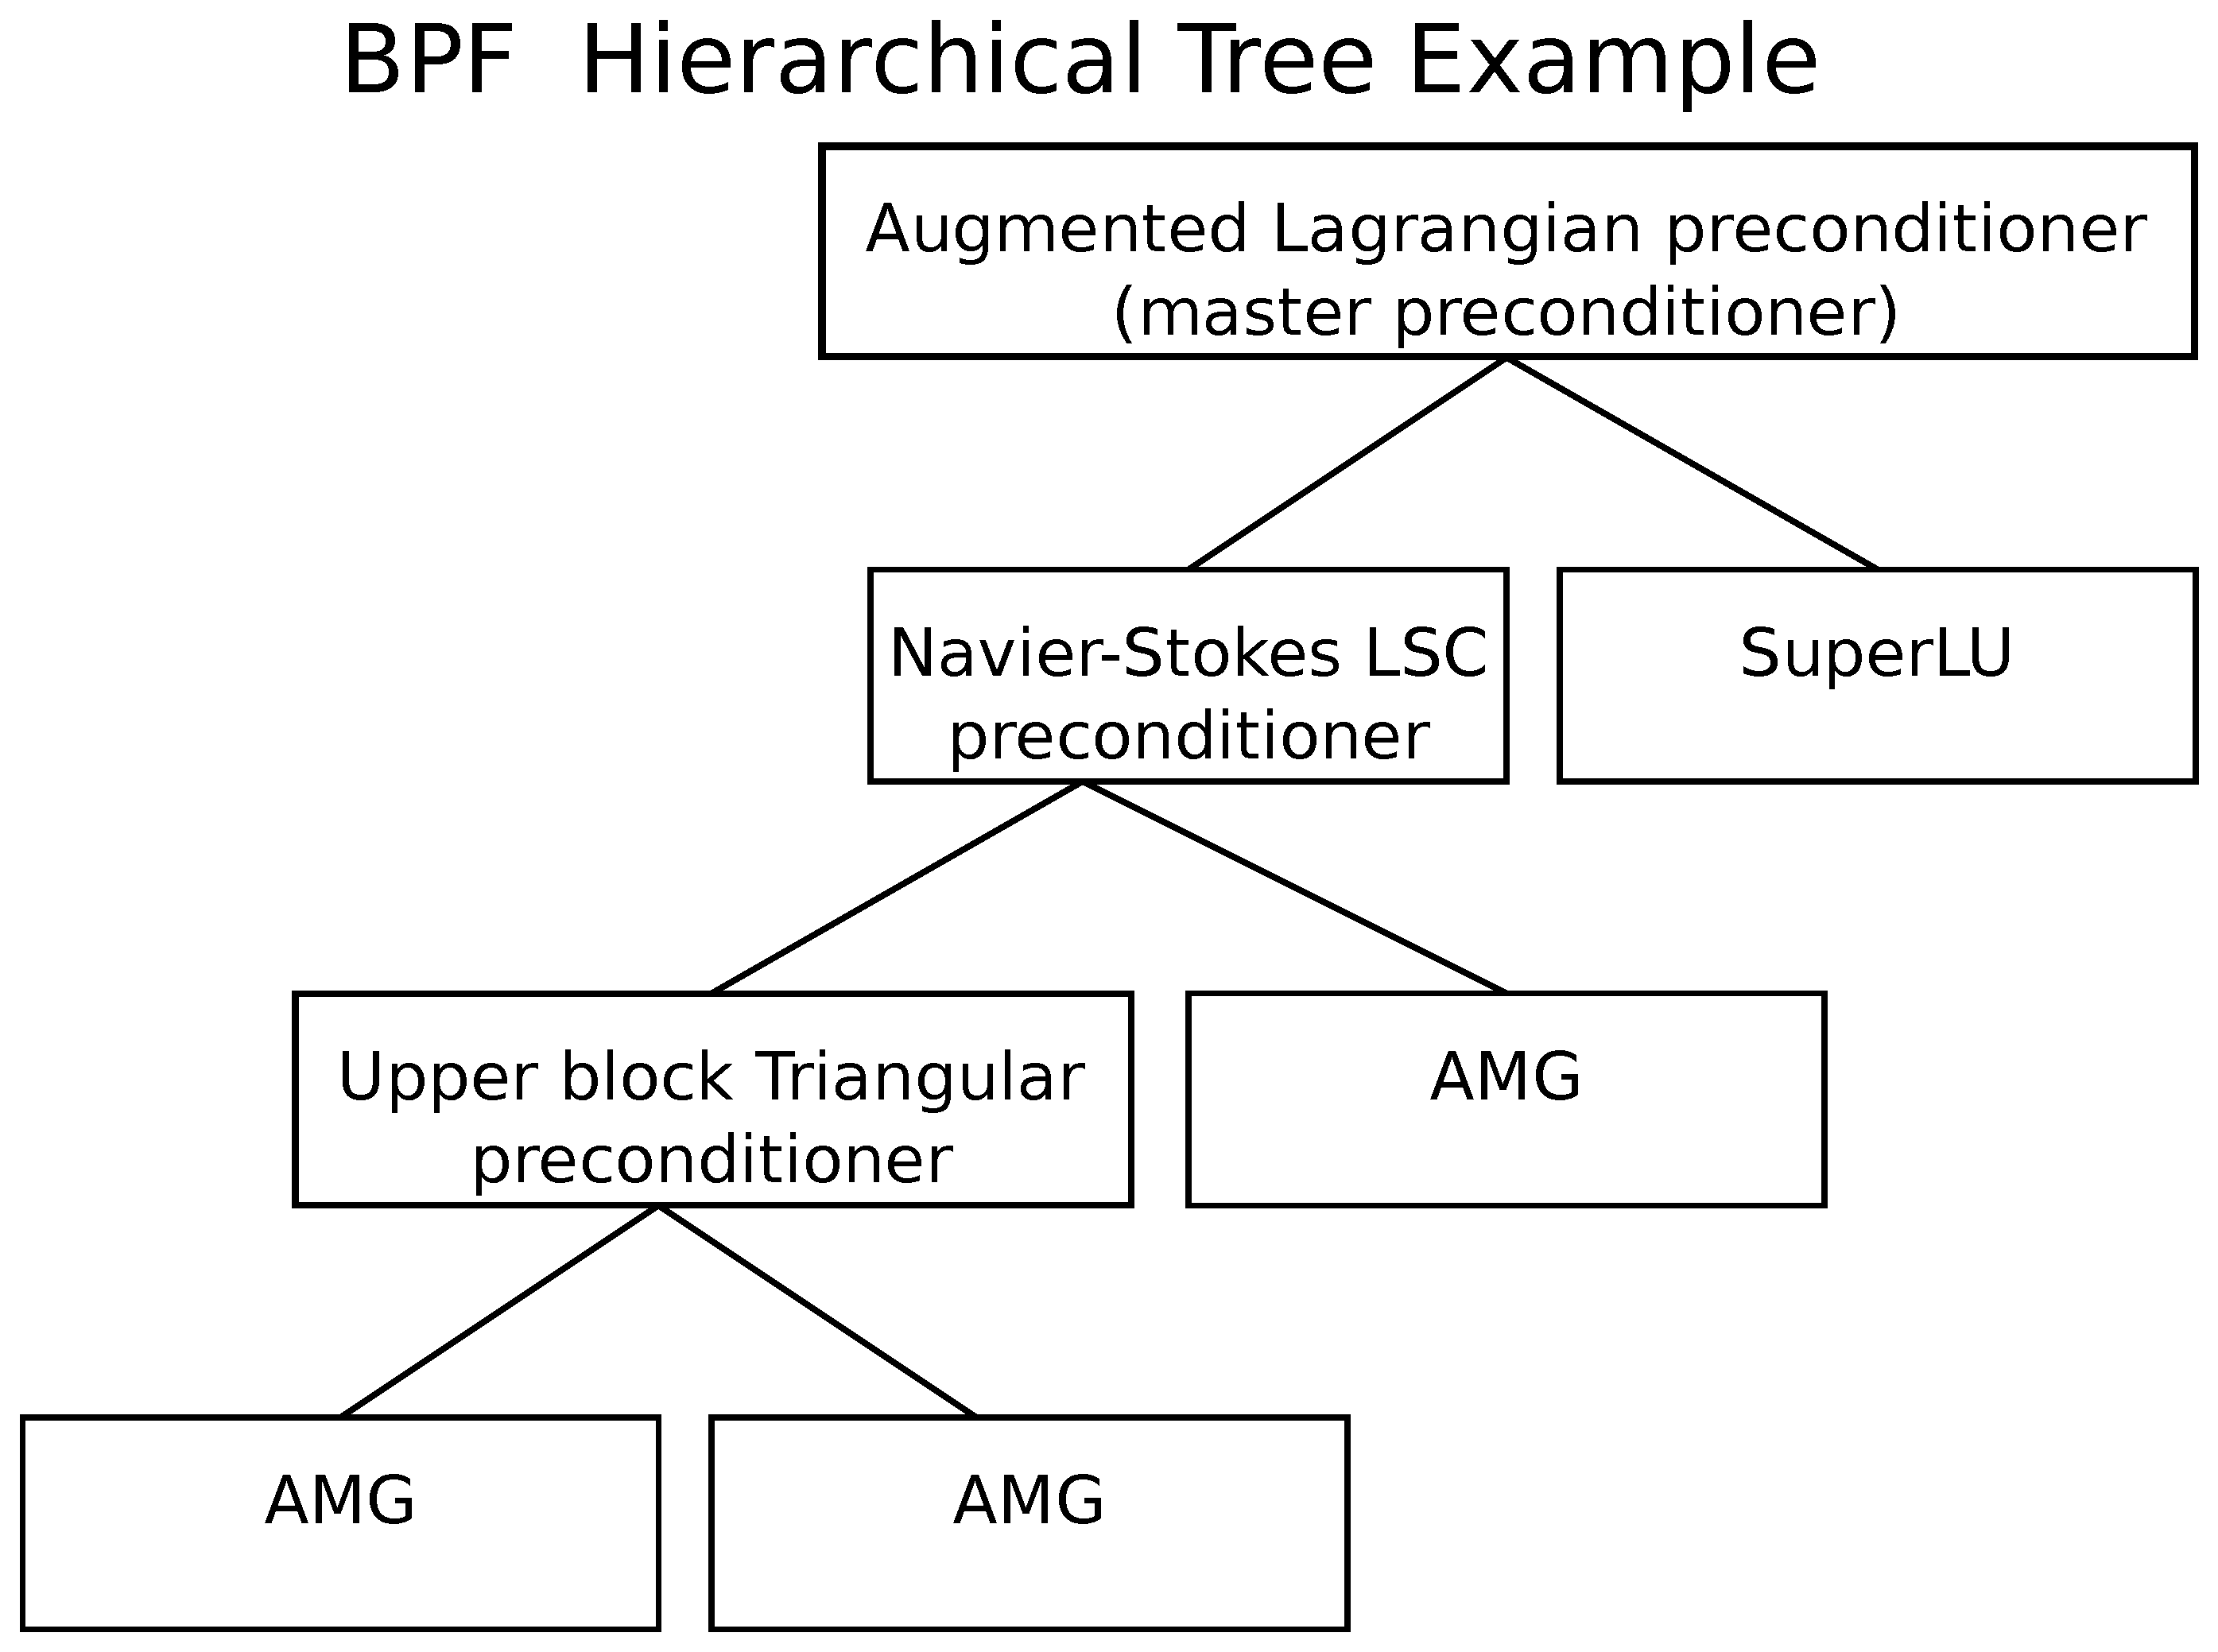
\includegraphics[width=0.8\textwidth]{./pic/bpf_hierarchy_tree_crop.pdf}
\caption{An example of a hierarchical tree resulting from multiple levels of
  subsidiary preconditioning. The master preconditioner is the Augmented
  Lagrangian preconditioner. When applying the master preconditioner, we can
  use existing preconditioners for the subsidiary systems, this process is
  depicted in Figure \ref{fig:bpf_hierarchy_matrixstructure_crop}.}
\label{fig:bpf_hierarchy_tree_crop}
\end{figure}

\begin{figure}[H]
\centering
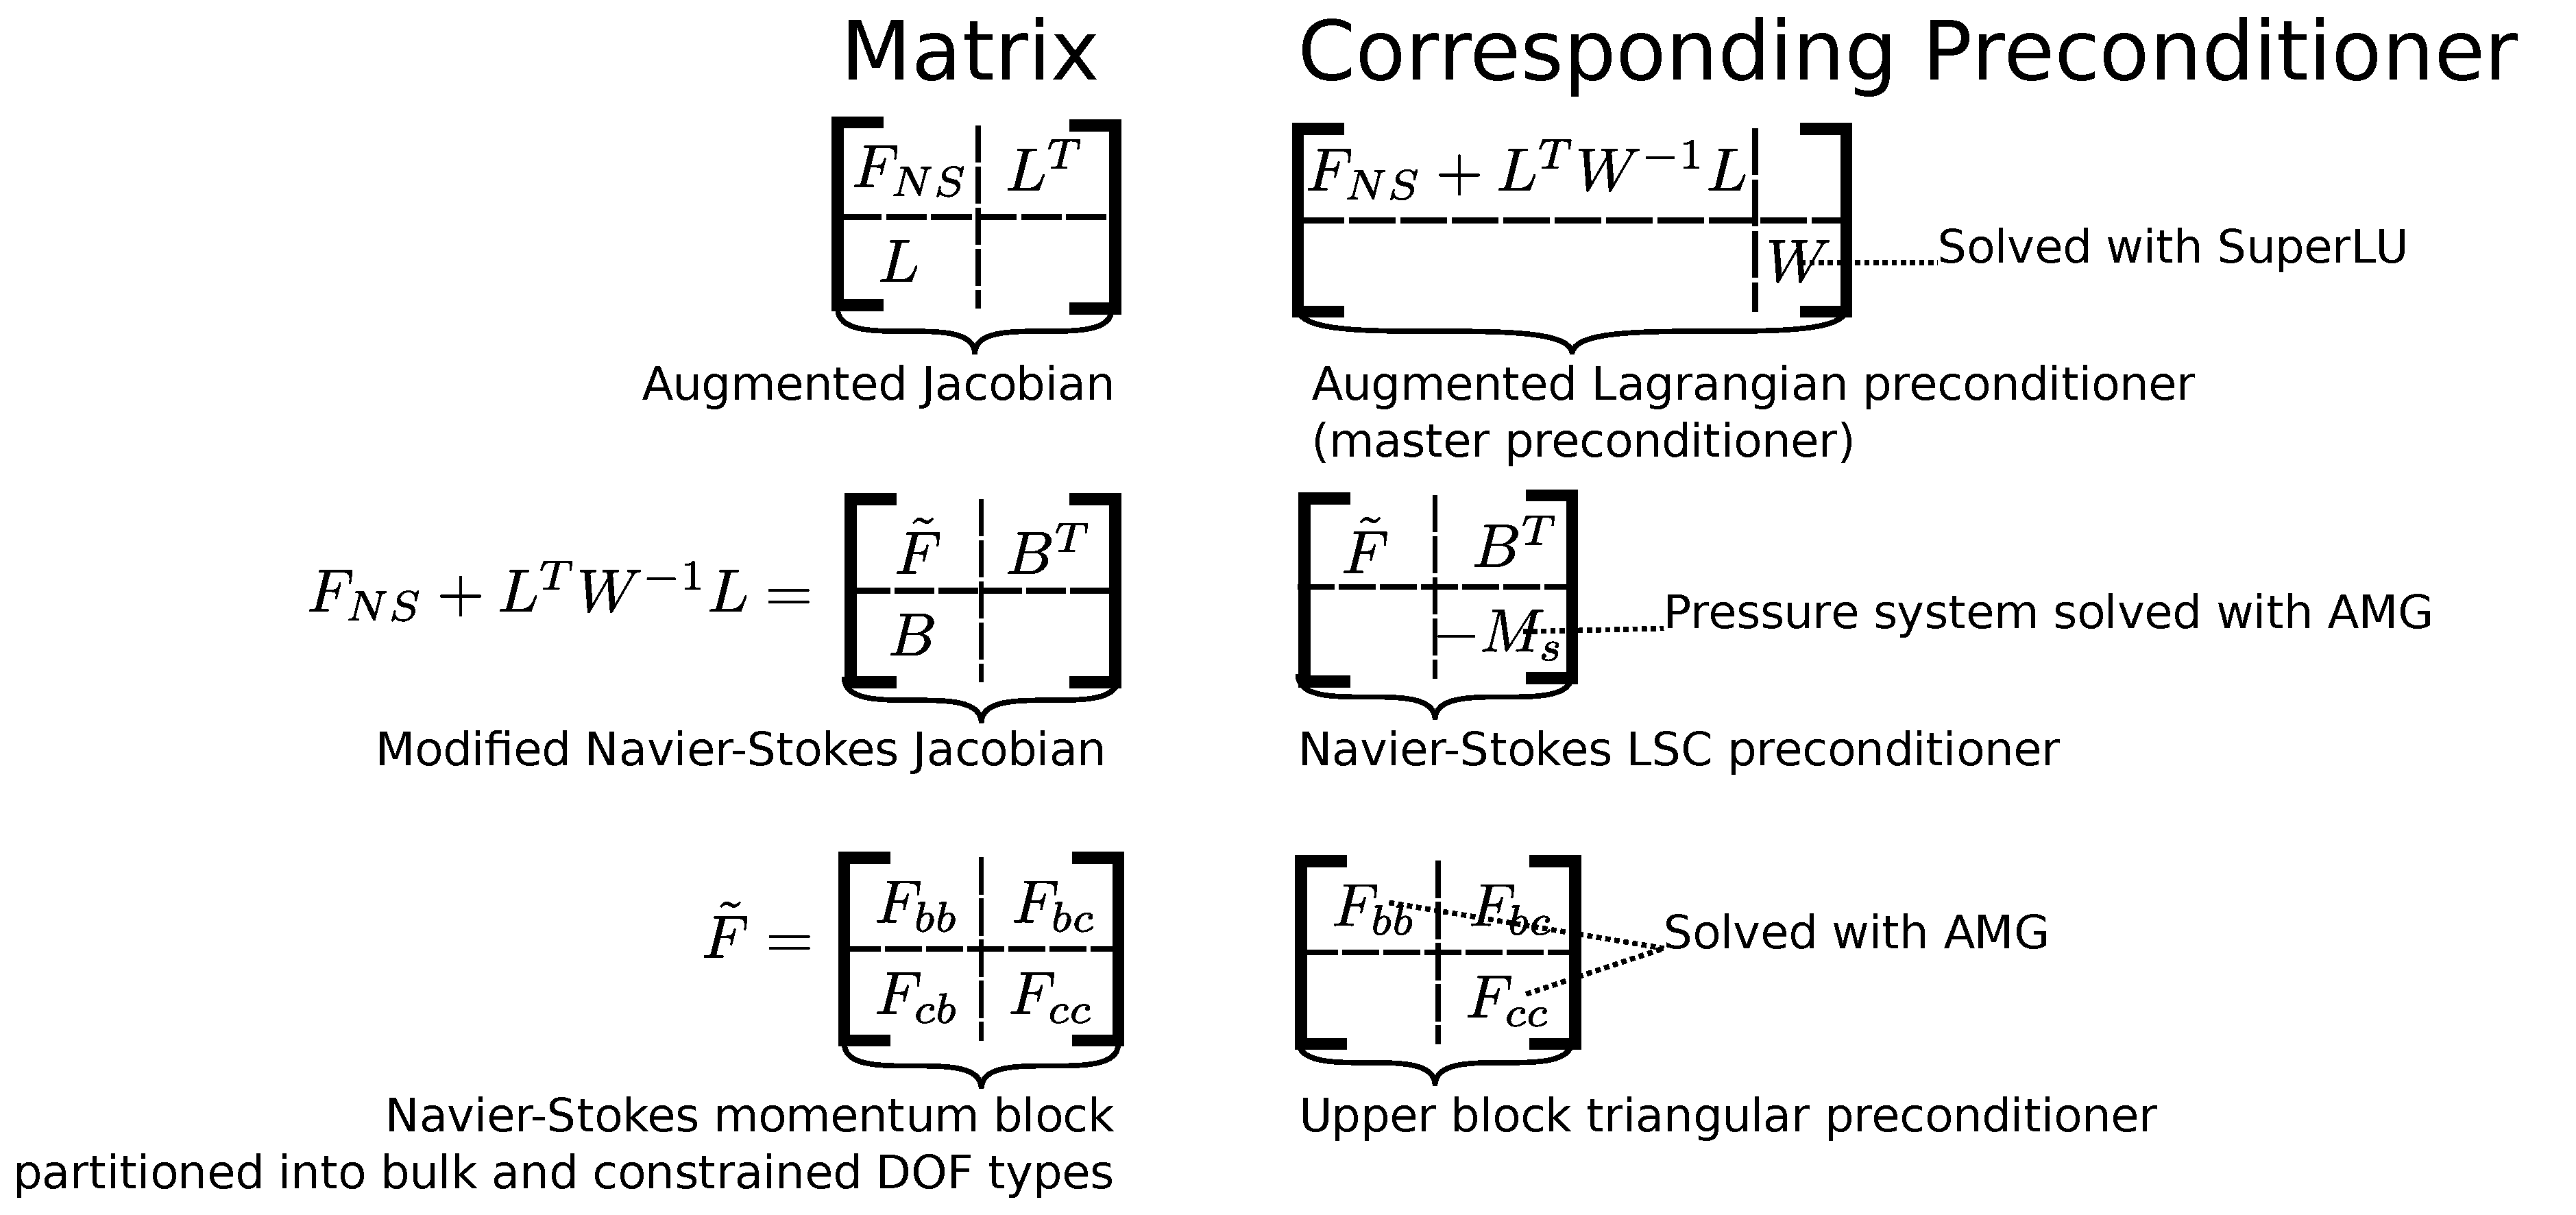
\includegraphics[width=1\textwidth]{./pic/bpf_hierarchy_matrixstructure_crop.pdf}
\caption{The structures of the matrices and corresponding preconditioners for
  the hierarchical tree structure presented in Figure
  \ref{fig:bpf_hierarchy_tree_crop}. The top left is the Jacobian resulting
  from Newton's method, to the right we have the corresponding Augmented
  Lagrangian preconditioner (see the matrices on the first row). The Augmented
  Lagrangian preconditioner requires the solution of two subsidiary systems, in
  particular, a modified Navier-Stokes subsystem. We can further approximate
  this subsystem with the Navier-Stokes LSC precondition (see the matrices on
  the second row). Applying Navier-Stokes LSC preconditioner requires the
  solution of the modified momentum block, which we can approximate with an
  upper block triangular preconditioner (see the third row).}
\label{fig:bpf_hierarchy_matrixstructure_crop}
\end{figure}

%Say, there are three
%preconditioners, $P1$, $P2$ and $P3$. If we use $P2$ to solve a subsidiary
%system in $P1$, and $P3$ to solve a subsidiary system in $P2$, then it could be
%said that $P1$ is the master preconditioner for $P2$, and $P2$ is a master
%preconditioner for $P3$. However, because $P2$'s \texttt{Master\_\allowbreak
%  block\_\allowbreak preconditioner\_\allowbreak pointer\_\allowbreak pt} is
%not null, it is automatically classed as a subsidiary preconditioner. Only the
%true master preconditioner (so that the \texttt{Master\_\allowbreak
%  block\_\allowbreak preconditioner\_\allowbreak pt} is null) holds all the
%information about the DOF types and look-up schemes. If a subsidiary
%preconditioner requires information held only by the master preconditioner, it
%will go to it's `master' preconditioner. If this `master' preconditioner is a
%subsidiary preconditioner, it will again go up the hierarchy to it's master
%preconditioner.

%%%%%%%%%%%%%%%%%%%%%%%%%%%%%%%%%%%%%%%%%%%%%%%%%%%%%
%%% USING THE SIMPLE DIAGONAL BLOCK PRECONDITIONER
%%%%%%%%%%%%%%%%%%%%%%%%%%%%%%%%%%%%%%%%%%%%%%%%%%%%%
\section{Using the Simple Block Preconditioner\label{sec:using_the_simple_block_preconditioner}}

We begin our discussion of the implementation details by demonstrating how to
use the preconditioner (implemented in the class \texttt{Simple\allowbreak
  Block\allowbreak Diagonal\allowbreak Preconditioner}) in an actual driver
code (\texttt{two\_\allowbreak d\_\allowbreak linear\_\allowbreak
  elasticity\_\allowbreak with\_\allowbreak simple\_\allowbreak
  block\_\allowbreak diagonal\_\allowbreak preconditioner\allowbreak
  .\allowbreak cc}).

In the problem constructor, we construct the solver and preconditioner
combination. We specify the GMRES iterative solver, and, if available, use the
distributed version implemented in \texttt{Trilinos\allowbreak Aztec\allowbreak
  OO\allowbreak Solver}.  \lstset{numberstyle=\scriptsize,breaklines=true,
  numbers=left, stepnumber=2, frame=single,basicstyle=\ttfamily\scriptsize,
  showstringspaces=false, language=C++} \lstinputlisting[firstnumber=348,
firstline=348,
lastline=361]{./code/two_d_linear_elasticity_with_simple_block_diagonal_preconditioner.cc}


Next we construct an instance of the preconditioner. Recall in Section
\ref{sec:framework_overview} that the order of the preconditioner DOF types is
determined by the elements, thus it is required that the preconditioner has
access to the elements which classify all the DOFs. This linear elasticity
problem contains one type of element used for preconditioning, i.e. the linear
elasticity elements should and do classify all the DOFs (see Section
\ref{sec:block_preconditionable_elements}). The linear elasticity elements are
stored in the so-called `bulk' mesh which is passed to the preconditioner via
two functions, \texttt{set\_\allowbreak nmesh(...)} \texttt{set\_\allowbreak
  mesh(...)}. 
\lstset{numberstyle=\scriptsize,breaklines=true, numbers=left, stepnumber=2, frame=single,basicstyle=\ttfamily\scriptsize, showstringspaces=false, language=C++}
\lstinputlisting[firstnumber=363,firstline=363, lastline=370]{./code/two_d_linear_elasticity_with_simple_block_diagonal_preconditioner.cc}
The function \texttt{set\_\allowbreak nmesh(...)} must be called before the
function \texttt{set\_\allowbreak mesh(...)} to let the BPF know how many
meshes there will be. Then we call the function \texttt{set\_\allowbreak
  mesh(...)} passing with the unsigned value \texttt{0} to indicate that the
\texttt{Mesh} should go in the first position and a pointer to the
\texttt{Mesh}. At the simplest level, \texttt{Mesh}es are regarded as
containers for elements. To reiterate
Section~\ref{sec:dof_types_and_block_types}, storing different element type in
separate meshes enables the BPF to differentiate between the elemental DOF
types of different element types. The tow-level ordering of the meshes and then
the elemental DOF types determine the order of the natural preconditioner DOF
types.  Therefore, in more sophisticated preconditioners, the preconditioner
usually handle the calls to \texttt{set\_\allowbreak nmesh(...)} and
\texttt{set\_\allowbreak mesh(...)} functions (see
Section~\ref{sec:lsc_block_preconditioner}). For this simplistic case, the
functions \texttt{set\_\allowbreak nmesh(...)} and \texttt{set\_\allowbreak
  mesh(...)} were called in the driver code. Passing the meshes to
\texttt{Block\allowbreak Preconditioner} gives the preconditioner read access
to the number of DOF types associated with the elements in each mesh which is
used to build the lookup schemes required to partition the matrix.

Finally, the preconditioner is passed to the solver.
\lstinputlisting[firstnumber=372,firstline=372, lastline=373]{./code/two_d_linear_elasticity_with_simple_block_diagonal_preconditioner.cc}

In the main function,
\lstset{numberstyle=\scriptsize,breaklines=true, numbers=left, stepnumber=2, frame=single,basicstyle=\ttfamily\scriptsize, showstringspaces=false, language=C++}
\lstinputlisting[firstnumber=450,firstline=450, lastline=454]{./code/two_d_linear_elasticity_with_simple_block_diagonal_preconditioner.cc}
we create an instance of the  problem which problem can now be solved in the
normal \texttt{oomph-\allowbreak lib} fashion:
\lstset{numberstyle=\scriptsize,breaklines=true, numbers=left, stepnumber=2, frame=single,basicstyle=\ttfamily\scriptsize, showstringspaces=false, language=C++}
\lstinputlisting[firstnumber=466,firstline=466, lastline=480]{./code/two_d_linear_elasticity_with_simple_block_diagonal_preconditioner.cc}

In the driver source code, you may notice \texttt{Linear\allowbreak
  Elasticity\allowbreak Traction\allowbreak Element}s. But the block
preconditioner does not need any information from these elements since the
elements in the bulk mesh already classify all the DOFs. We store the different
element types in different meshes. Only the bulk mesh is passed to the
preconditioner. 

%%%%%%%%%%%%%%%%%%%%%%%%%%%%%%%%%%%%%%%%%%%%%%%%%%%%%
%%% IMPLEMENTING A BLOCK DIAGONAL PRECONDITIONER
%%%%%%%%%%%%%%%%%%%%%%%%%%%%%%%%%%%%%%%%%%%%%%%%%%%%%
\section{The implementation of a block diagonal preconditioner\label{sec:the_implementation_of_a_block_diagonal_preconditioner}}

We discuss the implementation of a block diagonal preconditioner within
\texttt{oomph-\allowbreak lib}'s block preconditioning framework. In particular, we will
address three fundamental tasks: 
\begin{itemize} 
  \item How to identify and classify the DOFs in the underlying \texttt{Problem}.  
  \item How to extract subsidiary matrix blocks from the original matrix.
  \item How to reuse existing preconditioning operators within new preconditioners.
\end{itemize}

We implement the block diagonal preconditioner in the class
\texttt{Simple\allowbreak Block\allowbreak Diagonal\allowbreak Preconditioner}.
This class inherits from the base class \texttt{Block\allowbreak
  Preconditioner} which provides the generic functionality required for common
block preconditioning operations:
\lstset{numberstyle=\ttfamily\scriptsize,
        breaklines=true, 
        numbers=left, 
        stepnumber=2, 
        frame=single,
        basicstyle=\ttfamily\scriptsize, 
        showstringspaces=false, 
        language=C++}
\lstinputlisting[firstnumber=53,firstline=53, lastline=55]{./code/simple_block_preconditioners.h}
This preconditioner requires a \texttt{Vector} of pointers to \texttt{Preconditioner}s for each diagonal block matrix:
\lstinputlisting[firstnumber=97,firstline=97, lastline=99]{./code/simple_block_preconditioners.h}

%%%% CONSTRUCTOR FOR BLOCK DIAGONAL PRECONDITIONER
\subsection{Constructor for block diagonal preconditioner\label{sec:constructor_for_block_diagonal_preconditioner}}
The constructor is usually used to initialised variables. In this case, there is nothing to initialise:
\lstinputlisting[firstnumber=59,firstline=59, lastline=62]{./code/simple_block_preconditioners.h}
%%%% CONSTRUCTOR FOR BLOCK DIAGONAL PRECONDITIONER
\subsection{\texttt{setup(...)} for block diagonal preconditioner\label{sec:block_diagonal_preconditioner_setup}}

Like all preconditioners, \texttt{Block\allowbreak Preconditioners} have two
key functions, \texttt{setup(...)} and \texttt{preconditioner\_\allowbreak
  solve(...)} both of which are discussed in more detail in the
\texttt{oomph-\allowbreak lib} Linear Solvers Tutorial [CITE]. We begin by
considering the function \texttt{setup(...)}:
\lstinputlisting[firstnumber=107,firstline=107,lastline=109]{./code/simple_block_preconditioners.h} 
First we usually set the number of \texttt{Mesh}es via the function
\texttt{set\_\allowbreak nmesh(...)} and pass pointers to the \texttt{Mesh}es
via the function \texttt{set\_\allowbreak mesh(...)}. Since these two functions
were already invoked in the driver code, we can call the function
\texttt{block\_\allowbreak setup(...)} straight away.
\subsubsection{\texttt{block\_setup(...)}\label{sec:block_setup}}
The function \texttt{block\_\allowbreak setup(...)} creates the lookup scheme
between for the block types from a preconditioner DOF type to block type
mapping \texttt{Vector} and the ordering of the elemental and preconditioner
DOF types as described in Section~\ref{sec:dof_types_and_block_types}. To
define a mapping from the preconditioner DOF type to block type, we first look
at the structure of the matrix and the structure of the preconditioner. Since
we are designing a diagonal block preconditioner, we want the block type to be
as fine grained as the preconditioner DOF types. To see this, recall, if the
Jacobian (partitioned into preconditioner DOF types) takes the form 
\begin{equation}
J =
\begin{bmatrix}
J_{xx}&J_{xy} \\
J_{yx}&J_{yy}
\end{bmatrix},
\label{eq:simpleblockdiagonaljacobian}
\end{equation}
then a diagonal block preconditioner for \eqref{eq:simpleblockdiagonaljacobian}
is defined as
\begin{equation*}
P_{diag} =
\begin{bmatrix}
J_{xx}& \\
      &J_{yy}
\end{bmatrix}.
\label{eq:simpleblockdiagonalpreconditioner}
\end{equation*}
The preconditioner blocks from \eqref{eq:simpleblockdiagonalpreconditioner} are
as fine grained as the blocks from \eqref{eq:simpleblockdiagonaljacobian}, but
the matrix from \eqref{eq:simpleblockdiagonaljacobian} has been partitioned
into it's preconditioner DOF type. Thus the blocks the preconditioner works
with has to be as fine grained as the preconditioner DOF types. This is achieved
by calling the function \texttt{block\_\allowbreak setup(...)} with no
arguments. By default, this has the same effect as calling
\texttt{block\_\allowbreak setup(...)} with the identity
\texttt{dof\_\allowbreak to\_\allowbreak block\_\allowbreak map} \texttt{Vector
  \allowbreak =\allowbreak [0 1]}.
\lstinputlisting[firstnumber=111,firstline=111, lastline=112]{./code/simple_block_preconditioners.h}

For this simple block diagonal preconditioner, we have hard coded the
\texttt{dof\_\allowbreak to\_\allowbreak block\_\allowbreak map}
\texttt{Vector}. There exists a more sophisticated version of the block
diagonal preconditioner in the class \texttt{General\allowbreak
  Purpose\allowbreak Block\allowbreak Preconditioner}, where the function
\texttt{set\_\allowbreak dof\_\allowbreak to\_\allowbreak block\_\allowbreak
  map(Vector<unsigned>\& dof\_\allowbreak to\_\allowbreak block\_\allowbreak
  map)} can be called to change the \texttt{dof\_\allowbreak to\_\allowbreak
  block\_\allowbreak map} from the default. Below we describe how to use the \texttt{dof\_\allowbreak to\_\allowbreak block\_\allowbreak map}
\texttt{Vector} to re-order and combine preconditioner DOf types.

\subsubsection{\texttt{block\_setup(...)}: Combining DOF types\label{sec:block_setup_combining_dof_types}}
If we want a block type to consist of more than one preconditioner DOF type,
then we can provide a \texttt{dof\_\allowbreak to\_\allowbreak
  block\_\allowbreak map} to the function \texttt{block\_\allowbreak
  setup(...)} that describes which preconditioner DOF type to combine into one block type. For example, if we extend the
example above to three preconditioner DOF types,
\begin{equation*}
J =
\begin{bmatrix}
J_{xx}&J_{xy}&J_{xz} \\
J_{yx}&J_{yy}&J_{yz} \\
J_{zx}&J_{zy}&J_{zz}
\end{bmatrix},
\end{equation*}
and instead of simply using the diagonal blocks, we want to use a block
preconditioner of the following form
\begin{equation*}
\tilde{P}_{diag} =
\begin{bmatrix}
J_{xx}&J_{xy}&       \\
J_{yx}&J_{yy}&       \\
      &      &J_{zz}
\end{bmatrix},
\end{equation*}
that is, we want to group the first two preconditioner DOF types as one block
type and the last preconditioner DOF type as a separate block type. This is
achieved by passing the \texttt{dof\_\allowbreak to\_\allowbreak
  block\_\allowbreak map \allowbreak = \allowbreak [0 0 1]} to the function
\texttt{block\_\allowbreak setup(...)}, there is a similar
\texttt{dof\_\allowbreak to\_\allowbreak block\_\allowbreak map} that exists in
the implementation of the LSC preconditioner in
Section~\ref{sec:lsc_block_preconditioner}. It is important to notice that
although the $(0,0)$ block 
$\displaystyle
\begin{bmatrix}
S_{xx}&S_{xy} \\
S_{yx}&S_{yy} 
\end{bmatrix}
$
that contains two preconditioner DOF types $0$ and $1$, it is not guaranteed
that the grouping of the DOF types within the block is as intended.
\subsubsection{\texttt{block\_setup(...)}: Re-ordering DOF
  types\label{sec:block_setup_reordering_dof_types}} The natural ordering of
the preconditioner DOF types (based on the two-level ordering of the elemental
DOF types and the meshes as described in
Section~\ref{sec:dof_types_and_block_types}) is:
\begin{center}
    \begin{tabular}{ | r | c c c |}
    \hline
    DOF type name: & $S_{x}$ & $S_{y}$ & $S_{z}$ \\ 
    Natural ordering: & 0 & 1 & 2 \\ 
    \hline
    \end{tabular}
\end{center}
Suppose we want to re-order the DOF types such that we have the following block
order:
\begin{center}
    \begin{tabular}{ | r | c c c |}
    \hline
    New block order: & $S_{z}$ & $S_{x}$ & $S_{y}$ \\ 
    \hline
    \end{tabular}
\end{center}
Then the \texttt{dof\_\allowbreak to\_\allowbreak block\_\allowbreak map}
\texttt{Vector} will be
\begin{center}
    \begin{tabular}{ | r | c c c |}
    \hline
    \verb+dof_to_block_map+: & 1 & 2 & 0 \\ 
    \hline
    \end{tabular}
\end{center}
The index of the \texttt{dof\_\allowbreak to\_\allowbreak block\_\allowbreak
  map} \texttt{Vector} is the DOF type you want to move, then ask yourself
`where do I want to move this DOF type to?', put this value into the current
position in the \texttt{dof\_\allowbreak to\_\allowbreak block\_\allowbreak
  map} Vector.

Combining this with the previous concept, it is possible to create a preconditioner of the form
\begin{equation*}
\tilde{P}_{diag} =
\begin{bmatrix}
J_{zz}&J_{zx}&       \\
J_{xz}&J_{xx}&       \\
      &      &J_{yy}
\end{bmatrix}
\end{equation*}
with the \texttt{dof\_\allowbreak to\_\allowbreak block\_\allowbreak map}
\texttt{Vector} \texttt{[0 1 0]}.

%%%% Set up the subsidiary preconditioners
\subsubsection{Set up subsidiary preconditioners\label{sec:set_up_subsidiary_preconditioners}}
The next step is to set up the subsidiary preconditioners. We use the
\texttt{SuperLU} preconditioner as an exact solver for all the subsidiary
systems. As in each preconditioner we need to invert multiple subsidiary
preconditioners (as many as the number of blocks). First we create a new
instances of the of \texttt{SuperLU\allowbreak Preconditioner} for every block.
\lstinputlisting[firstnumber=114,firstline=114, lastline=124]{./code/simple_block_preconditioners.h}
Now we extract the diagonal blocks and call the \texttt{setup(...)} function for
the subsidiary preconditioners.
\lstinputlisting[firstnumber=126,firstline=126, lastline=138]{./code/simple_block_preconditioners.h}

%%%% PRECONDITIONER SOLVE FOR BLOCK DIAGONAL PRECONDITIONER
\subsection{\texttt{preconditioner\_solve(...)} for the block diagonal preconditioner\label{sec:preconditioner_solve_for_block_diagonal_preconditioner}}
Next we consider the \texttt{preconditioner\_\allowbreak solve(...)} function
which applies the action of the preconditioner to the input vector $\mathbf{y}$
(typically the linear residual at the current Krylov iteration) and returns the
result in $\mathbf{z}$.
\lstinputlisting[firstnumber=142,firstline=142, lastline=147]{./code/simple_block_preconditioners.h}
In this section, we implement the application of the preconditioner as
described in Section~\ref{sec:theoretical_background}. First invoke the
function \texttt{get\_\allowbreak block\_\allowbreak vectors(...)} which splits
the rhs vector into sub-vectors and re-arranged (permute) them to match the
block order of the preconditioner blocks.
\lstinputlisting[firstnumber=149,firstline=149, lastline=152]{./code/simple_block_preconditioners.h}
Next we loop through the LU decompositions stored in the
\texttt{Diagonal\_\allowbreak block\_\allowbreak preconditioner\_\allowbreak
  pt}, and apply the subsidiary preconditioners via back substitution.
\lstinputlisting[firstnumber=157,firstline=157, lastline=163]{./code/simple_block_preconditioners.h}
Finally we copy the solution back into $\mathbf{z}$ in the correct DOF order.
\lstinputlisting[firstnumber=165,firstline=165, lastline=166]{./code/simple_block_preconditioners.h}



%%%%%%%%%%%%%%%%%%%%%%%%%%%%%%%%%%%%%%%%%%%%%%%%%%%%%%
%%%% LSC BLOCK PRECONDITIONER
%%%%%%%%%%%%%%%%%%%%%%%%%%%%%%%%%%%%%%%%%%%%%%%%%%%%%%
\section{LSC block preconditioner\label{sec:lsc_block_preconditioner}}
Theoretical discussion of the LSC preconditioner can be found in "Finite
Elements and Fast Iterative Solvers with Applications in Incompressible Fluid
Dynamics" by Howard C. Elman, David J. Silvester, and Andrew J. Wathen,
published by Oxford University Press, 2006.

In this section, we partially follow the \texttt{oomph-lib} LSC tutorial [CITE
oomph-lib lsc tutorial], where we take a closer look at the implementation
details to address the following concepts:
\begin{itemize}
\item Non trivial grouping of preconditioner DOF types into block types.
\item Setting up \texttt{Matrix\allowbreak Vector\allowbreak Product}s within the block preconditioning framework.
\item Subsidiary block preconditioners:
 \begin{itemize}
 \item The \texttt{dof\_\allowbreak map} for the \texttt{turn\_\allowbreak into\_\allowbreak subsidiary\_\allowbreak block\_\allowbreak preconditioner(...)} function.
 \item Modification to the \texttt{preconditioner\_\allowbreak solve(...)} function.
 \end{itemize}
\end{itemize}

%%%% LSC theory
\subsection{Theory (background)\label{sec:lsc_theory}}
\texttt{oomph-\allowbreak lib} currently provides two types of (LBB-stable)
Navier-Stokes elements: Taylor-Hood (Q2-Q1) and Crouzeix-Raviart (Q2-Q-1)
elements. These contain two distinct types of degrees of freedom, namely the
velocities and pressures.

The least-squares commutator Navier-Stokes preconditioner employs
\texttt{oomph-\allowbreak lib}'s block-preconditioning framework to (formally)
re-order the linear system to be solved during the Newton iteration into 2x2
blocks, corresponding to the velocity and pressure unknowns. We note that all
velocity components are treated as a single block of unknowns. The linear
system therefore has the following block structure
\begin{equation}
\begin{bmatrix}
{\bf F} & {\bf G} \\ {\bf D} & {\bf 0} 
\end{bmatrix}
\begin{bmatrix}
{\bf z}_u \\ {\bf z}_p
\end{bmatrix} 
 =
\begin{bmatrix}
{\bf r}_u \\ {\bf r}_p
\end{bmatrix} 
.
\label{eq:NS_jacobian}
\end{equation}
Here $\mathbf{F}$ is the momentum block, $\mathbf{G}$ the discrete gradient
operator, and $\mathbf{D}$ the discrete divergence operator. (For unstabilised
elements, we have $\mathbf{D} = \mathbf{G}^T$ and in much of the literature the
divergence matrix is denoted by $\mathbf{B}$.)

An "exact" preconditioner would solve this system exactly and thus ensure the
convergence of any iterative linear solver in a single iteration. However, the
application of such a preconditioner would, of course, be asymptotically as
expensive as a direct solve.  The LSC preconditioner replaces the exact
Jacobian by a block-triangular approximation
\begin{equation*}
\begin{bmatrix}
{\bf F} & {\bf G} \\ {\bf 0} & -{\bf M}_s 
\end{bmatrix} 
\begin{bmatrix}
{\bf z}_u \\ {\bf z}_p
\end{bmatrix} 
=
\begin{bmatrix}
{\bf r}_u \\ {\bf r}_p
\end{bmatrix}
,
\end{equation*}
where $\mathbf{M}_s$ is an approximation to the pressure 
Schur-complement $\mathbf{S}=\mathbf{D} \mathbf{F}^{-1}\mathbf{G}$.
This system can be solved in two steps:
\begin{enumerate}
\item Solve the second row for $\mathbf{z}_p$ via
   \begin{equation*}
   \mathbf{z}_p = - \mathbf{M}_s^{-1} \mathbf{r}_p
   \end{equation*}
\item Given $\mathbf{ z}_p$, solve the first row for $\mathbf{z}_u$ via
   \begin{equation*}
   \mathbf{z}_u = \mathbf{F}^{-1} \left( \mathbf{r}_u - \mathbf{G} \mathbf{z}_p \right)
   \end{equation*}
\end{enumerate}
In the LSC preconditioner, the action of the inverse pressure
Schur complement 
\begin{equation*}
\mathbf{z}_p = - \mathbf{M}_s^{-1} \mathbf{r}_p
\end{equation*}
is approximated by
\begin{equation*}
\mathbf{z}_p = - 
\big(\mathbf{D} \widehat{\mathbf Q}^{-1}{\mathbf G} \big)^{-1}
\big({\mathbf D} \widehat{\mathbf Q}^{-1}{\mathbf F} \widehat{\mathbf Q}^{-1}{\mathbf G}\big) 
\big({\mathbf D} \widehat{\mathbf Q}^{-1}{\mathbf G} \big)^{-1}
{\mathbf r}_p,
\end{equation*}
where  $ \widehat{\mathbf Q}$ is the diagonal of the velocity
mass matrix. The evaluation of this expression involves
two linear solves involving the matrix
\begin{equation*}
{\mathbf P} = \big({\mathbf D} \widehat{\mathbf Q}^{-1}{\mathbf G} \big)
\end{equation*}
which has the characteristics of a matrix arising from the discretisation of a
Poisson problem on the pressure space. We also have to evaluate matrix-vector
products with the matrix 
\begin{equation*}
{\mathbf E}={\mathbf D}\widehat{\mathbf Q}^{-1}{\mathbf F}\widehat{\mathbf Q}^{-1}{\mathbf G},
\end{equation*}
these are achieved by successive sparse matrix-vector multiplications.
In our implementation of the preconditioner, the linear systems
can either be solved "exactly", using \texttt{SuperLU} (in its incarnation
as an exact preconditioner; this is the default) or approximately by any 
other \texttt{Preconditioner} (interpreted as an "inexact solver")
specified via the access functions
\begin{verbatim}
NavierStokesSchurComplementPreconditioner::set_f_preconditioner(...)
\end{verbatim}
or 
\begin{verbatim}
NavierStokesSchurComplementPreconditioner::set_p_preconditioner(...)
\end{verbatim}

%%%% Implementation details
\subsection{Implementation details\label{sec:lsc_implementation}}
In this section we focus on implementation details of the LSC preconditioner in the context of the BPF. Let \texttt{dim} be the
spatial dimension of the problem, then \texttt{Navier\allowbreak
  Stokes\allowbreak Schur\allowbreak Complement\allowbreak Preconditioner}
expects \texttt{dim + 1} preconditioner DOF types, \texttt{dim} number of DOF
types for the velocity and 1 DOF type for the pressure. 

\subsubsection{\texttt{setup(...)} for the LSC preconditioner\label{sec:lsc_implementation_setup}}
We need to combine the velocity DOF types into one \emph{block type} and the
pressure DOF type as one block type. This is achieved by setting the first
\texttt{dim} entries of the \texttt{dof\_\allowbreak to\_\allowbreak block\_\allowbreak map}
\texttt{Vector} to 0 and the last entry to 1.
\lstinputlisting[firstnumber=235,firstline=235, lastline=238]{./code/navier_stokes_preconditioners.cc}
For example, in two dimensions, the natural ordering of the DOF types and the
\texttt{dof\_\allowbreak to\_\allowbreak block\_\allowbreak map \allowbreak Vector} is given below.
\begin{center}
    \begin{tabular}{ | r | c c c |}
    \hline
    DOF type name: & $u$ & $v$ & $p$ \\ 
    Natural ordering: & 0 & 1 & 2 \\ 
    \texttt{dof\_\allowbreak to\_\allowbreak block\_\allowbreak map}: & 0 & 0 & 1 \\ 
    \hline
    \end{tabular}
\end{center}
The implementation follows the theory in section \ref{sec:lsc_theory}. In the
sequel we highlight some important implementation details. 

When setting up a \texttt{Matrix\allowbreak Vector\allowbreak Product}, it is
important to use the setup function \texttt{setup\_\allowbreak
  matrix\_\allowbreak vector\_\allowbreak product(...)}.  The first argument is
a pointer to the \texttt{Matrix\allowbreak Vector\allowbreak Product}, the
second is a pointer to the matrix, the third is an unsigned value indicating
the block vector operand. This ensures that the column distribution of the
\texttt{Matrix\allowbreak Vector\allowbreak Product} is set up properly:
\lstinputlisting[firstnumber=507,firstline=507, lastline=508]{./code/navier_stokes_preconditioners.cc}

If the $\mathbf{F}$ preconditioner is a block preconditioner (used to solve the
system $\mathbf{z}_u = \mathbf{F}^{-1} \left( \mathbf{r}_u - \mathbf{G}
  \mathbf{z}_p \right)$), then we must call the function
\texttt{turn\_\allowbreak into\_\allowbreak subsidiary\_\allowbreak
  block\_\allowbreak preconditioner(...)} of the $\mathbf{F}$ preconditioner.
This function takes the pointer of the `master' preconditioner (in the sense
that the master preconditioner is just one level higher in the block
preconditioning framework hierarchy), and a \texttt{Vector} describing a
mapping of preconditioner DOF types of the master preconditioner and the
subsidiary preconditioner. Then the \texttt{setup(...)} function of the
subsidiary preconditioner is called with a pointer to the original Jacobian
(via the access function \texttt{matrix\_\allowbreak pt()}). If the
$\mathbf{F}$ preconditioner is not a block preconditioner, then we do the same
as we did in the simple block diagonal preconditioner case:
\lstinputlisting[firstnumber=589,firstline=589, lastline=612]{./code/navier_stokes_preconditioners.cc}
The \texttt{dof\_\allowbreak map} Vector is different from the
\texttt{dof\_\allowbreak to\_\allowbreak block\_\allowbreak map}
\texttt{Vector}.  The \texttt{dof\_\allowbreak to\_\allowbreak
  block\_\allowbreak map} \texttt{Vector} describes the mapping of the
preconditioner DOF types to block types within the same block preconditioner.
As such, this \texttt{Vector} must have the same size as the number of DOF
types the preconditioner expects it works with (applies to). The
\texttt{dof\_\allowbreak map} \texttt{Vector} describes the mapping between the
DOF types of a master preconditioner with it's subsidiary preconditioner.
Re-ordering DOF types of the subsidiary preconditioner using the
\texttt{dof\_\allowbreak map} \texttt{Vector} is possible and will be
demonstrated in the implementation of the augmented Lagrangian preconditioner
discussed later in this document.


\subsubsection{\texttt{preconditioner\_solve(...)} for the LSC preconditioner\label{sec:lsc_implementation_precsolve}}
The \texttt{preconditioner\_\allowbreak solve(...)} function for the LSC
preconditioner follows the approach discussed in Section~\ref{sec:lsc_theory}.
When block preconditioner are used as subsidiary preconditioners, we DO NOT
return the block vector, as this is handled by the subsidiary block
preconditioner.
\lstinputlisting[firstnumber=801,firstline=801, lastline=812]{./code/navier_stokes_preconditioners.cc}


%%%%%%%%%%%%%%%%%%%%%%%%%%%%%%%%%%%%%%%%%%%%%%%%%%%%%
%%% LAGRANGIAN BLOCK PRECONDITIONER
%%%%%%%%%%%%%%%%%%%%%%%%%%%%%%%%%%%%%%%%%%%%%%%%%%%%%
\section{Augmented Lagrangian block preconditioner\label{sec:lagrangian_block_preconditioner}}
In this section, we use the implementation of the Lagrangian preconditioner to
address the following concepts:
\begin{itemize}
\item Non-trivial re-ordering of block types.
\item Non-trivial re-ordering of subsidiary DOF types.
\item Set precomputed preconditioner blocks for subsidiary block
  preconditioners.
\end{itemize}
As with previous examples, we highlight the key concepts and neglect the finer
implementation details of the preconditioner for the specific problem. The code
is (as always) well documented and can be worked through with the theory at
hand.
%%%% LSC theory
\subsection{Theory background\label{sec:lgr_theory}}
Consider the problem of imposing no-slip or parallel axially traction free
outflow boundary conditions for flow problems defined on arbitrarily shaped
domains. One convenient way of imposing BCs in such cases is by using Lagrange
multipliers [CITE]. For example, to impose parallel axially traction free
outflow along part of the boundary, we need to attach the block
preconditionable elements \texttt{Impose\allowbreak Parallel\allowbreak
  Outflow\allowbreak Element} along that part of the boundary as discussed in
Section~\ref{sec:dof_types_and_block_types}. This will result in a Jacobian of
the following block form (partitioned by DOF types):
\renewcommand{\arraystretch}{1.2}
\begin{equation}
\newcommand*{\temp}{\multicolumn{1}{r|}{}}
\left[
\begin{array}{cccccccc}
F_{xx}&F_{xy}&F_{x\hat{x}}&F_{x\hat{y}}& \temp &(B_x)^T&\temp & \\ 
F_{yx}&F_{yy}&F_{y\hat{x}}&F_{y\hat{y}}& \temp &(B_{y})^T&\temp & \\
F_{\hat{x}x}&F_{\hat{x}y}&F_{\hat{x}\hat{x}}&F_{\hat{x}\hat{y}}& \temp &(B_{\hat{x}})^T&\temp & M_x\\
F_{\hat{y}x}&F_{\hat{y}y}&F_{\hat{y}\hat{x}}&F_{\hat{y}\hat{y}}& \temp &(B_{\hat{y}})^T&\temp &M_y \\ 
  \cline{1-7}
B_x&B_{y} &B_{\hat{x}} &B_{\hat{y}} & \temp &  &\temp & \\ 
  \cline{1-8}
  & & M_x & M_y&       &  &\temp & \\
\end{array}
\right]
\left[
\begin{array}{c}
\delta \bar{u}_x \\
\delta \bar{u}_y \\
\delta \bar{u}_{\hat{x}} \\
\delta \bar{u}_{\hat{y}} \\
\delta \bar{p} \\
\delta \bar{l} \\
\end{array}
\right]
=
\left[
\begin{array}{c}
\delta \bar{r}_x \\
\delta \bar{r}_y \\
\delta \bar{r}_{\hat{x}} \\
\delta \bar{r}_{\hat{y}} \\
\delta \bar{r}_p \\
\delta \bar{r}_l \\
\end{array}
\right],
\end{equation}
\renewcommand{\arraystretch}{1}
where the block vector $[\bar{u}_x \, \bar{u}_{\hat{x}}]^T$ contains the unknown $x$-velocity component. Similarly, the block vector
$[\bar{u}_y \, \bar{u}_{\hat{y}}]^T$ contains the unknown $y$-velocity component. The hat represents the nodes at the constrained boundary affected by the Lagrange
multiplier constraint. The Lagrange multiplier block takes the form
\begin{equation*}
	L =
\begin{bmatrix}
 O & O & M_x & M_y & O \\
\end{bmatrix}.
\end{equation*}
For simplicity, we can re-write the Jacobian as
\begin{equation*}
	\mathcal{J} = 
	\begin{bmatrix}
	 \mathcal{F} & L\\
	L & \mathit{O}
	\end{bmatrix},
\end{equation*}
where $\mathcal{F}$ is he whole Navier-Stokes system \eqref{eq:NS_jacobian}.
For this saddle point problem, we seek an augmented preconditioner of the form
\begin{equation*}
	\mathcal{P} = 
	\begin{bmatrix}
	 \mathcal{F}+ L^T W^{-1} L & \mathit{O}\\
	\mathit{O} & W
	\end{bmatrix}
\end{equation*}
The matrix $W\in \mathbb{R}^{n_l \times n_l}$ is chosen to be
 \begin{equation}
 	W = 
 	\begin{bmatrix}
 	\frac{1}{\sigma}L L^T
 	\end{bmatrix},
 	\label{eq:W}
 \end{equation}
to preserve the sparsity of $\mathcal{F}$ and $\sigma$ is chosen to be the norm
of the momentum block to be an effective preconditioner for the above saddle
point problem[REFERENCE ANALYSIS TO JUSTIFY CHOICE]. The application of this preconditioner requires the approximate solution of the
two principal diagonal blocks. We can further approximate the augmented
$\hat{\mathcal{F}} = \mathcal{F} + L^TW^{-1}L$ block by the LSC approximation.
This is facilitated by the re-use of block preconditioners in
\texttt{oomph-\allowbreak lib}'s block preconditioning framework.

Detailed theoretical discussion for the Lagrangian preconditioner can be found in [CITE some chapter in my thesis or the yet to be published paper].
%%%% Implementation details
\subsection{Implementation details\label{sec:lgr_implementation}}

The Lagrangian preconditioner takes the `bulk' mesh as the first mesh (the mesh containing the TaylorHood elements). Subsequent meshes are surfaces meshes containing the \texttt{Impose\allowbreak Parallel\allowbreak Outflow\allowbreak Element} elements. We have established in Section \ref{sec:dof_types_and_block_types} that this leads to the natural DOF type ordering
\begin{center}
    \begin{tabular}{ | r | c c c c c c |}
    \hline
    DOF type name:    & $u$ & $v$ & $p$ & $u_c$ & $v_c$ & $L$ \\ 
    Natural ordering: & 0   &  1  &  2  &   3   &   4   &  5  \\ 
    \hline
    \end{tabular}
\end{center}
Where $u$ and $v$ are the `bulk' velocity DOF types in the $x$ and $y$
direction, $u_c$ and $v_c$ are the constrained velocity DOF types in the $x$
and $y$ direction DOF type, $p$ is the pressure DOF type and $L$ is the
Lagrange multiplier DOF type. 


 \subsubsection{\texttt{setup(...)} for the Lagrangian preconditioner\label{sec:lgr_setup}}
First we need to create the \texttt{dof\_\allowbreak to\_\allowbreak
  block\_\allowbreak map} to create the block ordering as discussed in
Section~\ref{sec:lgr_theory}. Recall from \ref{sec:dof_types_and_block_types}
that to re-order block types, we ask ourselves `where do I want to move this
DOF type to?'. This leads to the following \texttt{dof\_\allowbreak
  to\_\allowbreak block\_\allowbreak map}:
\begin{center}
    \begin{tabular}{ | r | c c c c c c |}
    \hline
    DOF type name:      & $u$ & $v$ & $p$ & $u_c$  & $v_c$ & $L$ \\ 
    Natural ordering:   & 0   &  1  &  2  &   3    &   4   &  5  \\ 
Desired block ordering: & $u$ & $v$ & $u_c$ & $v_c$& $p$   & $L$ \\ 
\texttt{dof\_to\_block\_map}:& 0   &  1  &  4  &   2    &   3   &  5  \\
    \hline
    \end{tabular}
\end{center}
The creation of the \texttt{dof\_\allowbreak to\_\allowbreak block\_\allowbreak
  map} \texttt{Vector} is generalised to multiple surface meshes in the
\texttt{setup(...)} function of the \texttt{Lagrange\allowbreak
  Enforcedflow\allowbreak Preconditioner} class:
\lstinputlisting[firstnumber=1078,firstline=1078, lastline=1101]{./code/lagrange_enforced_flow_preconditioner.h}

Suppose want to use the LSC block preconditioner to approximate the
$\hat{\mathcal{F}}$. First we need to create the \texttt{dof\_\allowbreak map}
which describes which DOF types from the Lagrangian preconditioner that the LSC
preconditioner works with. We have to work with the DOF types from the natural
order and ask ourselves `which DOF type from the master preconditioner do I
want to move into this position?'. The \texttt{dof\_\allowbreak map} for this
problem is given below, along with the \texttt{dof\_\allowbreak to\_\allowbreak
  block\_\allowbreak map} for comparison.
\begin{center}
    \begin{tabular}{ | r | c c c c c c |}
    \hline
    DOF type name:      & $u$ & $v$ & $p$ & $u_c$  & $v_c$ & $L$ \\ 
    Natural ordering:   & 0   &  1  &  2  &   3    &   4   &  5  \\ 
Desired block ordering: & $u$ & $v$ & $u_c$ & $v_c$& $p$   & $L$ \\ 
\texttt{dof\_to\_block\_map}:& 0   &  1  &  4  &   2    &   3   &  5  \\
\texttt{dof\_map}:         & 0   &  1  &  3  &   4    &   2   &     \\
    \hline
    \end{tabular}
\end{center}
For the \texttt{Lagrange\allowbreak Enforcedflow\allowbreak Preconditioner},
the \texttt{dof\_\allowbreak map} generation is generalised to work with
multiple surface meshes:
\lstinputlisting[firstnumber=1003,firstline=1003, lastline=1034]{./code/lagrange_enforced_flow_preconditioner.h}
The above code actually generates the list \texttt{[0 1 3 4 2 5]}, where the first \texttt{dim*nmesh} entries corresponds to the $\mathcal{F}$ DOF types. Therefore we fill the \texttt{dof\_\allowbreak map} with only the required DOF types:
\lstinputlisting[firstnumber=1704,firstline=1704, lastline=1708]{./code/lagrange_enforced_flow_preconditioner.h}
Then we proceed to call the \texttt{turn\_\allowbreak into\_\allowbreak subsidiary\_\allowbreak block\_\allowbreak preconditioner(...)} function:
\lstinputlisting[firstnumber=1733,firstline=1733, lastline=1735]{./code/lagrange_enforced_flow_preconditioner.h}

There exists two problems if we want to re-use the LSC block preconditioner:
\begin{enumerate}
\item The LSC preconditioner expects \texttt{dim \allowbreak + \allowbreak 1}
  DOF types. In our case Navier-Stokes block consists of \texttt{dim*nmesh
    \allowbreak + \allowbreak 1} DOF types.
\item The function \texttt{get\_\allowbreak block(...)} extracts the block
  matrix from the original Jacobian. We want the LSC preconditioner to operate
  on the modified $\hat{\mathcal{F}}$ block.
\end{enumerate}
There exists one function to solve both problems. The function
\texttt{set\_\allowbreak precomputed\_\allowbreak blocks(...)} takes a
\texttt{Dense\allowbreak Matrix} consisting of pointers to the (possibly
modified) precomputed preconditioner blocks and (yet another!) mapping
(\texttt{dof\_\allowbreak to\_\allowbreak dof\_\allowbreak map}) between the
DOF types of the master preconditioner and the subsidiary preconditioner. This
mapping describes which DOF type of the master preconditioner should be treated
as a single DOF type in the subsidiary preconditioner.  For the above example,
the \texttt{dof\_\allowbreak to\_\allowbreak dof\_\allowbreak map}
\texttt{Vector} would be the two dimension \texttt{Vector}:
\begin{verbatim}
0 [0 2]
1 [1 3]
2 [4]
\end{verbatim}
Recall that we now have the DOF type ordering
\begin{center}
    \begin{tabular}{ | r | c c c c c c |}
    \hline
                        & 0   &  1  &  2  &   3    &   4   &  5  \\ 
Desired block ordering: & $u$ & $v$ & $u_c$ & $v_c$& $p$   & $L$ \\ 
    \hline
    \end{tabular}
\end{center}
so the \texttt{dof\_\allowbreak to\_\allowbreak dof\_\allowbreak map} says to
the LSC preconditioner `treat DOF types 0 and 2 from the master preconditioner
as DOF type 0, treat the DOF types 1 and 3 from the master preconditioner as
DOF type 1, and treat DOF type 4 from the master preconditioner as DOF type 2'.
Again, the implementation of the \texttt{Lagrange\allowbreak
  Enforcedflow\allowbreak Preconditioner} is fully generalised, but will
produce the above results.

In the below code, we fill the \texttt{f\_\allowbreak subblock\_\allowbreak pt} with the (modified) velocity blocks and the rest of the pressure block $B$ to form the blocks required for $\hat{\mathcal{F}}$:
The code below describes how we create the \texttt{dof\_\allowbreak to\_\allowbreak dof\_\allowbreak map}:
\lstinputlisting[firstnumber=1747,firstline=1747, lastline=1767]{./code/lagrange_enforced_flow_preconditioner.h}
Now, we set the precomputed blocks and call \texttt{setup(...)}:
\lstinputlisting[firstnumber=1769,firstline=1769, lastline=1773]{./code/lagrange_enforced_flow_preconditioner.h}

%%%%%%%%%%%%%%%%%%%%%%%%%%%%%%%%%%%%%%%%%%%%%%%%%%%%%
%%% Source files
%%%%%%%%%%%%%%%%%%%%%%%%%%%%%%%%%%%%%%%%%%%%%%%%%%%%%
\section{Source Files\label{sec:source_files}}
The following source files were used for our discussion of \verb+oomph-lib+'s block preconditioning framework.

\noindent
{\scriptsize
\verb+demo_drivers/linear_solvers/two_d_linear_elasticity_with_simple_block_diagonal_preconditioner.cc+
}

\noindent
{\scriptsize
\verb+demo_drivers/linear_solvers/simple_block_preconditioners.h+
}

\noindent
{\scriptsize
\verb+src/navier_stokes/navier_stokes_preconditioners.h+
}

\noindent
{\scriptsize
\verb+src/navier_stokes/navier_stokes_preconditioners.cc+
}

\noindent
{\scriptsize
\verb+src/navier_stokes/lagrange_enforced_flow_preconditioner.h+
}

%%%%%%%%%%%%%%%%%%%%%%%%%%%%%%%%%%%%%%%%%%%%%%%%%%%%%
%%% Source files
%%%%%%%%%%%%%%%%%%%%%%%%%%%%%%%%%%%%%%%%%%%%%%%%%%%%%
%\section{Under the hood\label{sec:under_the_hood}}
%In this section we take a closer look at innards of the block preconditioning framework. In particular, the mechanism for setting precomputed preconditioner blocks. This feature was developed to allow the re-use of block preconditioners when the master preconditioner has modified the preconditioner blocks. This knowledge is not required for developing new preconditioners, but it may be useful for maintaining the block preconditioning framework.
%
%The following discussion assumes good knowledge of the distributed data structures used within \verb+oomph-lib+, in particular, how data is distributed. If you are not already familiar with these concepts, please refer to the \verb+oomph-lib+ tutorials `Parallel processing' and `Distributed Linear Algebra infrastructure'.
%
%\texttt{Block\-Preconditioner}s are \texttt{Distributed\-Linear\-Algebra\-Object}s. Their \texttt{Linear\-Algebra\-Distribution} can be accessed via the function \texttt{preconditioner\-\_matrix\-\_distribution\-\_pt()}. This \texttt{Linear\-Algebra\-Distribution} describes the distribution of the preconditioner, which is the concatenation of inidividual block distributions \emph{without communication}.
%
%The concatenation of \texttt{Distributed\-Linear\-Algebra\-Object}s without communication means to `combine' several objects (of the same type) into a new object whilst keeping the data on the processor it already resides. For reference, see the following functions:
%\begin{itemize}
%\item \texttt{CRDoubleMatrixHelpers::concatenate\_without\_communication(...)}
%\item \texttt{DoubleVectorHelpers::concatenate\_without\_communication(...)}
%\item \texttt{LinearAlgebraDistributionHelpers::concatenate(...)}
%\end{itemize}
%
%The distributions of the inidividual preconditioner blocks are uniformly distributed. However, the distribution of the preconditioner (which is a concatenation of the distributions of it's preconditioner blocks) is not uniformly distributed. This means one cannot generate a uniformly distributed matrix and use it as a preconditioner within a particular preconditioner, since the preconditioner expects the preconditioner matrix to have the same distribution as the concatenation of the distributions of the individual preconditioner blocks.
%
%The distribution of the individual preconditioner blocks is stored within each block preconditioner and can be accessed via the function \texttt{block\-\_distribution\-\_pt(...)}.
%
%\subsection{Setting precomputed preconditioner blocks\label{sec:setting_precomputed_preconditioner_blocks}}
%
%We revisit the Lagrangian block preconditioner example discussed in section \ref{sec:lagrangian_block_preconditioner} and assume we have a two dimensional problem with one bulk mesh containing \texttt{QTaylor\-Hood\-Element}s and one surface mesh containing \texttt{Impose\-Parallel\-Outflow\-Element}s. After re-ordering the block types as discribed in section \ref{sec:lgr_implementation}, we have the following block order:
%\begin{center}
%    \begin{tabular}{ | r | c c c c c c |}
%    \hline
%                        & 0   &  1  &  2  &   3    &   4   &  5  \\ 
%Desired block ordering: & $u$ & $v$ & $u_c$ & $v_c$& $p$   & $L$ \\ 
%    \hline
%    \end{tabular}
%\end{center}
%The blocks corresponding to the constrained velocities, namely blocks (2,2), (2,3), (3,2) and (3,3) have been modified by the Lagrangian preconditioner. We want to apply the LSC preconditioner to the (modified) Navier-Stokes blocks 0-4, so we pass pointers to these blocks to the LSC preconditioner.
%
%Within the LSC preconditioner (which splits the block types into velocity and pressure), when we call \texttt{get\-\_block(0,0)}, the preconditioning framework would know that preconditioner blocks have been precomputed and will return a concatenation (without communication) of the following blocks
%\begin{equation*}
%\begin{bmatrix}
%(0,0) & (0,2) & (0,1) & (0,3) \\
%(2,0) & (2,2) & (2,1) & (2,3) \\
%(1,0) & (1,2) & (1,1) & (1,3) \\
%(3,0) & (3,2) & (3,1) & (3,3)
%\end{bmatrix}.
%\end{equation*}
%Since the concatenation is without communication, the distribution of the resuling block(0,0) is not uniform. But the inidivual blocks of a preconditioner always have a uniform distribution! More importantly, this mean that the block vector 0 from the LSC preconditioner also have a uniform distribution, so we cannot use the above preconditioner block since it's distribution is different from that of the vector we with to apply the matrix operation to.
%
%We ensure that the distribution of the preconditioner block matrix is the same as the distribution of the vector we wish to apply the matrix to by the following method: If preconditioner blocks have been precomputed then
%\begin{itemize}
%\item use the identity \texttt{dof\-\_to\-\_block\-\_map} for the \texttt{bloc\-k\_setup(...)} function.
%\item when the function \texttt{get\-\_block(...)} is called, use the lookup scheme set by \texttt{dof\-\_to\-\_dof\-\_map} to concatenate the relevant \emph{precomputed} preconditioner blocks (without communication).
%\item when the function \texttt{get\-\_block\-\_vector(...)} is called, use the lookup scheme set by \texttt{dof\-\_to\-\_dof\-\_map} to extract the relevant block vector and concatenate  them (without communication).
%\item when the function \texttt{return\-\_block\-\_vector(...)} is called, split the vector into the relevant block vectors and return each block vector back to the vector we wish to return the entries to.
%\end{itemize}
%As long as the precomputed preconditioner blocks are ordered in the same manner as the underlaying blocks of the LSC preconditioner (the subsidiary preconditioner), then the distribution is the same for the concatenated precomputed block and the concatenated block vectors. The order of the underlaying blocks of the subsidiary preconditioner is determined by the \texttt{dof\-\_map} vector passed to the function \texttt{turn\-\_into\-\_subsidiary\-\_block\-\_preconditioner(...)}.
%
%This scheme has a few RAYRAYsubtitles:
%\begin{itemize}
%\item If preconditioner blocks have been precomputed for a preconditioner, then the number of block types for the preconditioner is the most fine grain. This means that the number of preconditioner DOF types equal to the number of block types.
%\item The function \texttt{nblock\-\_types(...)} still returns the number of block types the preconditioner expects without precomputed preconditioner blocks.
%\item The function \texttt{ndof\-\_types(...)} still returns the number of DOF types the preconditioner expects without precomputed preconditioner blocks.
%\end{itemize}
%
%\subsection{Limitations and future development\label{sec:limitations_and_future_development}}
%There is no mechanism to split a matrix which has been concatenated (with or without communication). This means, if the LSC preconditioner was to modify it's preconditioner blocks (having already been set precomputed preconditioner blocks from a master preconditioner), there is no way (yet!) to split up the matrices into the most fine grain block type to pass them down to a another subsidiary preconditioner. The current scheme only allows for one preconditioner in the \emph{hierarchical chain} to modify the preconditioner blocks and pass them down to subsidiary block preconditioners. Two subsidiary block preconditioners can modify the preconditioner blocks and pass them down to it's own subsidiary preconditioner(s) if they are operating on completely different subsidiary systems.
%
%There exists another approach to the whole problem. When the preconditioner blocks are modified by the master preconditioner and to be used by a subsidiary block  preconditioner, the master preconditioner copies the entries back into a copy of the Jacobian. Thus we do not have to concatenate the precomputed block matrices nor do we have to always work with the most fine grain block type. Implementation of this feature was considered but due to time constraints, was not implemented; there is currently no book keeping information of where the DOF came from and there would still be the problem of combining DOF types in the subsidiary preconditioner.
%
%\newpage
%
%%
%%\begin{equation}
%%P_{NS} = 
%%\begin{bmatrix}
%% F & B^T \\
%%\mathit{O} & -M_S
%%\end{bmatrix}.
%%\label{eq:NSgeneralprec}
%%\end{equation}
%
%
